% ---------------------------------------------------------------------------
% Author guideline and sample document for EG publication using LaTeX2e input
% D.Fellner, v1.13, Jul 31, 2008

\documentclass{egpubl}
\usepackage{eurovis2016}

% --- for  Annual CONFERENCE
% \ConferenceSubmission   % uncomment for Conference submission
% \ConferencePaper        % uncomment for (final) Conference Paper
% \STAR                   % uncomment for STAR contribution
% \Tutorial               % uncomment for Tutorial contribution
% \ShortPresentation      % uncomment for (final) Short Conference Presentation
% \Areas                  % uncomment for Areas contribution
% \MedicalPrize           % uncomment for Medical Prize contribution
% \Education              % uncomment for Education contribution
%
% --- for  CGF Journal
% \JournalSubmission    % uncomment for submission to Computer Graphics Forum
% \JournalPaper         % uncomment for final version of Journal Paper
%
% --- for  CGF Journal: special issue
% \SpecialIssueSubmission    % uncomment for submission to Computer Graphics Forum, special issue
\SpecialIssuePaper         % uncomment for final version of Journal Paper, special issue
%
% --- for  EG Workshop Proceedings
% \WsSubmission    % uncomment for submission to EG Workshop
% \WsPaper         % uncomment for final version of EG Workshop contribution
%
 \electronicVersion % can be used both for the printed and electronic version

% !! *please* don't change anything above
% !! unless you REALLY know what you are doing
% ------------------------------------------------------------------------

% for including postscript figures
% mind: package option 'draft' will replace PS figure by a filname within a frame
\ifpdf \usepackage[pdftex]{graphicx} \pdfcompresslevel=9
\else \usepackage[dvips]{graphicx} \fi

\PrintedOrElectronic

% prepare for electronic version of your document
\usepackage{t1enc,dfadobe}

\usepackage{egweblnk}
\usepackage{cite}

% For backwards compatibility to old LaTeX type font selection.
% Uncomment if your document adheres to LaTeX2e recommendations.
% \let\rm=\rmfamily    \let\sf=\sffamily    \let\tt=\ttfamily
% \let\it=\itshape     \let\sl=\slshape     \let\sc=\scshape
% \let\bf=\bfseries

% end of prologue

%%%%%%%%%%%%%%%%%%%%%%%%%%%%%%%%%%%%%%%%%%%%%%%%%%%%
%\documentclass[review,journal]{vgtc}          % review (journal style)
%\documentclass[widereview]{vgtc}             % wide-spaced review
%\documentclass[preprint,journal]{vgtc}       % preprint (journal style)
%\documentclass[electronic,journal]{vgtc}     % electronic version, journal
\let\ifpdf\relax

%% Uncomment one of the lines above depending on where your paper is
%% in the conference process. ``review'' and ``widereview'' are for review
%% submission, ``preprint'' is for pre-publication, and the final version
%% doesn't use a specific qualifier. Further, ``electronic'' includes
%% hyperreferences for more convenient online viewing.

%% Please use one of the ``review'' options in combination with the
%% assigned online id (see below) ONLY if your paper uses a double blind
%% review process. Some conferences, like IEEE Vis and InfoVis, have NOT
%% in the past.

%% Please note that the use of figures other than the optional teaser is not permitted on the first page
%% of the journal version.  Figures should begin on the second page and be
%% in CMYK or Grey scale format, otherwise, colour shifting may occur
%% during the printing process.  Papers submitted with figures other than the optional teaser on the
%% first page will be refused.

%% These three lines bring in essential packages: ``mathptmx'' for Type 1
%% typefaces, ``graphicx'' for inclusion of EPS figures. and ``times''
%% for proper handling of the times font family.

% Math-mode symbol & verbatim
\def\W#1#2{$#1{#2}$ &\tt\string#1\string{#2\string}}
\def\X#1{$#1$ &\tt\string#1}
\def\Y#1{$\big#1$ &\tt\string#1}
\def\Z#1{\tt\string#1}

\usepackage{mathptmx}
%%\usepackage{psfrag}
\usepackage{graphicx}
\usepackage{times}
\usepackage{epstopdf}

%\usepackage{amssymb,amsmath,amsthm}
\usepackage{amssymb,amsmath}
\usepackage[lined,linesnumbered]{algorithm2e}
\usepackage{caption}
\usepackage{subcaption}
\usepackage{multirow}
\usepackage{framed}
\usepackage{tikz}
%\usepackage{array}

\usepackage{float}

\usepackage{varwidth}

%% We encourage the use of mathptmx for consistent usage of times font
%% throughout the proceedings. However, if you encounter conflicts
%% with other math-related packages, you may want to disable it.

%% This turns references into clickable hyperlinks.
%%\usepackage[bookmarks,backref=true,linkcolor=black]{hyperref} %,colorlinks
%% \hypersetup{
%%  pdfauthor = {},
%%  pdftitle = {},
%%  pdfsubject = {},
%%  pdfkeywords = {},
%%  colorlinks=true,
%%  linkcolor= black,
%%  citecolor= black,
%%  pageanchor=true,
%%  urlcolor = black,
%%  plainpages = false,
%%  linktocpage
%%}

%% If you are submitting a paper to a conference for review with a double
%% blind reviewing process, please replace the value ``0'' below with your
%% OnlineID. Otherwise, you may safely leave it at ``0''.
%%\onlineid{0}

%% declare the category of your paper, only shown in review mode
%%\vgtccategory{Technique}

%% allow for this line if you want the electronic option to work properly
%%\vgtcinsertpkg

%% In preprint mode you may define your own headline.
%\preprinttext{To appear in an IEEE VGTC sponsored conference.}


%%%%%%%%%%%%%%%%%%%%%%%%%%%%%%%%%%%%%%%%%%%%%%%%%%%%%%%%%%%%%%%%%%%%%%%%%%%%%
%
% Math commands
%
%%%%%%%%%%%%%%%%%%%%%%%%%%%%%%%%%%%%%%%%%%%%%%%%%%%%%%%%%%%%%%%%%%%%%%%%%%%%%

\newcommand {\emath}[1]  {\ensuremath{#1}}
\newcommand {\R}         {\emath{\mathbb{R}}}        % Real space
\newcommand {\Real}[1]   {\emath{\mathbb{R}^{#1}}}   % Real space
\newcommand {\Rd}        {\Real{d}}                  % R^d
\newcommand {\Rdone}     {\Real{d+1}}                % R^d+1
\newcommand {\Rk}        {\Real{k}}                  % R^k
\newcommand {\Rtwo}      {\Real{2}}                  % R^2
\newcommand {\Rthree}    {\Real{3}}                  % R^3
\newcommand {\Rfour}     {\Real{4}}                  % R^4
\newcommand {\Sphere}[1] {\emath{\mathbb{S}^{#1}}}   % Sphere
\newcommand {\Sk}        {\Sphere{k}}                % S^k
\newcommand {\Sd}        {\Sphere{d}}                % S^d
\newcommand {\BB}        {\emath{\mathbb{B}}}        % B
\newcommand {\Ball}[1]   {\emath{\mathbb{B}^{#1}}}   % B^{#1}
\newcommand {\Ballep}    {\emath{B^{\epsilon}_{p}}}  % B^e_p
\newcommand {\cl}        {\emath{\mathrm{cl}}}       % cl
\newcommand {\cb}        {\emath{\mathbf{c}}}        % bold c
\newcommand {\eb}        {\emath{\mathbf{c}}}        % bold e
\newcommand {\tpi}       {\emath{\tilde{\pi}}}       % \pi~
\newcommand {\gDim}[1]   {\emath{#1 \times #1 \times #1}} % DxDxD

\newcommand {\tg}        {\emath{\tilde{g}}}
\newcommand {\tn}        {\emath{\tilde{n}}}
\newcommand {\IV}        {\emath{\mathcal{I_V}}}
\newcommand {\Orth}      {\emath{\mathcal{O}}}
\newcommand {\hN}        {\emath{\widehat{N}}}
\newcommand {\XX}        {\emath{\mathcal{X}}}

\newtheorem{proposition}{Proposition}
\newtheorem{corollary}{Corollary}[proposition]
\newtheorem{lemma}[proposition]{Lemma}


%%%%%%%%%%%%%%%%%%%%%%%%%%%%%%%%%%%%%%%%%%%%%%%%%%%%%%%%%%%%%%%%%%%%%%%%%%%%%
%
% tikz block styles
%
%%%%%%%%%%%%%%%%%%%%%%%%%%%%%%%%%%%%%%%%%%%%%%%%%%%%%%%%%%%%%%%%%%%%%%%%%%%%%

\usetikzlibrary{shapes,arrows}

\tikzstyle{action} = [rectangle, draw, text centered, node distance=4cm, minimum height=4em]
\tikzstyle{source} = [draw, ellipse, text centered, node distance=1.5cm, minimum height=4em, text width=3cm]
\tikzstyle{sink} = [draw, ellipse, text centered, node distance=2cm, minimum height=4em]
\tikzstyle{line} = [draw, -latex']
\tikzstyle{figlabel} = [text centered, node distance=1.5cm, text width=1cm]

% Define block styles
\tikzstyle{decision} = [diamond, draw, fill=white!20, text width=4.5em, text badly centered, node distance=3cm, inner sep=0pt]
\tikzstyle{block} = [rectangle, draw,thick,fill=blue!0, text centered, rounded corners, minimum height=1em]
\tikzstyle{cloud} = [draw, ellipse,fill=red!20, node distance=3cm,minimum height=2em]

%%%%%%%%%%%%%%%%%%%%%%%%%%%%%%%%%%%%%%%%%%%%%%%%%%%%%%%%%%%%%%%%%%%%%%%%%%%%%
%
% algorithm2e keywords and commands
%
%%%%%%%%%%%%%%%%%%%%%%%%%%%%%%%%%%%%%%%%%%%%%%%%%%%%%%%%%%%%%%%%%%%%%%%%%%%%%

% algorithm2e global keywords
\SetKw{Function}{Function}
\SetKw{true}{true}
\SetKw{false}{false}
\SetKw{KwAnd}{and}
\SetKw{KwOr}{or}
\SetKw{true}{true}
\SetKw{false}{false}
\SetKw{KwElse}{else}
\SetKw{KwDownTo}{downto}
\SetKwData{NULL}{NULL}
\SetKwInOut{Input}{Input}
\SetKwInOut{Output}{Output}
\SetKwInOut{Result}{Result}
\SetKwInOut{Requires}{Requires}
\ResetInOut{Requires1}
\SetKwComment{NoLineNum}{}{}
\SetCommentSty{textit}
\SetArgSty{textrm}
\SetFuncSty{textsc}
\SetAlgoLined

\IncMargin{1ex}

\SetKwFunction{AngleTest}{AngleTest}
\SetKwFunction{ScalarTest}{ScalarTest}
\SetKwFunction{ReliableGrad}{ReliableGrad}
\SetKwFunction{MergeSharp}{MergeSharp}
\SetKwFunction{FindSharp}{FindSharp}
\SetKwFunction{CountDegree}{CountDegree}
\SetKwFunction{SelectiveFindSharp}{SelectiveFindSharp}
\SetKwFunction{Magnitude}{Magnitude}
\SetKwFunction{Angle}{Angle}
\SetKwFunction{Distance}{Distance}
\SetKwData{Grid}{Grid}
\SetKwData{numAgree}{numAgree}
\SetKwData{errorDist}{errorDist}
\SetKwData{maxErrorDist}{maxErrorDist}
\SetKwData{numIter}{numIter}

% Algorithm function names and variables
\SetKwFunction{DoesOrthMatch}{DoesOrthMatch}
\SetKwFunction{DoesOrthMatchA}{DoesOrthMatchA}
\SetKwFunction{DoesOrthMatchB}{DoesOrthMatchB}
\SetKwFunction{ExtendReliable}{ExtendReliable}


\SetKwData{Center}{Center}
\SetKwData{Centroid}{Centroid}
\SetKwData{isovLoc}{isovLoc}
\SetKwData{numLargeEigenvalues}{numLargeEigenvalues}

% algorithm2e reset line number
\newcommand {\ResetAlgoLineNumber} {\setcounter{AlgoLine}{0}}

\SetAlgoCaptionSeparator{.}


\title{Visualizing flow fields using fractal dimensions}

%% This is how authors are specified in the journal style

%% indicate IEEE Member or Student Member in form indicated below
\author{Ross Vasko, Han-Wei Shen and Rephael Wenger}
%%\authorfooter{
%%The Ohio State University. E-mail: vasko.38@osu.edu, shen.94@osu.edu
%% and wenger.4@osu.edu}

\begin{document}

\maketitle

\begin{abstract}
Streamlines are a popular way of visualizing flow in vector fields.
A major challenge in streamline visualization is selecting the streamlines
for visualization.
Rendering too many streamlines clutters the visualization and makes
features of the field difficult to identify. 
Rending too few streamlines causes viewers to completely miss features
of the flow field not rendered. 

The fractal dimension of a streamline represents its space-filling properties.
To identify complex or interesting streamlines, 
we build a regular grid of scalar values 
which represent the fractal dimension of streamlines around each grid vertex.
High fractal dimension indicates vortices or turbulent regions.
We use this scalar grid both to filter streamlines by fractal dimension
and to identify and visualize regions containing vortices and turbulence.
We describe an interactive tool which allows for quick streamline selection
and visualization of regions containing vortices and turbulence.
\end{abstract}

%% Keywords that describe your work. Will show as 'Index Terms' in journal
%% please capitalize first letter and insert punctuation after last keyword
%\keywords{Streamlines, fractal dimension.}

%% ACM Computing Classification System (CCS). 
%% See <http://www.acm.org/class/1998/> for details.
%% The ``\CCScat'' command takes four arguments.

%%\CCScatlist{ % not used in journal version
%%\CCScat{I.3.5}{Computer Graphics}{Computational Geometry and Object Modeling}
%%}

%% Uncomment below to include a teaser figure.
%\teaser{
%}

%% Uncomment below to disable the manuscript note
%\renewcommand{\manuscriptnotetxt}{}

%% Copyright space is enabled by default as required by guidelines.
%% It is disabled by the 'review' option or via the following command:
% \nocopyrightspace

\renewcommand{\textfraction}{0.2}
\renewcommand{\dbltopfraction}{0.8}	
\renewcommand{\topfraction}{0.8}	


%%%%%%%%%%%%%%%%%%%%%%%%%%%%%%%%%%%%%%%%%%%%%%%%%%%%%%%%%%%%%%%%
%%%%%%%%%%%%%%%%%%%%%% START OF THE PAPER %%%%%%%%%%%%%%%%%%%%%%
%%%%%%%%%%%%%%%%%%%%%%%%%%%%%%%%%%%%%%%%%%%%%%%%%%%%%%%%%%%%%%%%%

%%\maketitle

\section{Introduction}

A vector field in 3D is a map $f: \Rthree \Rightarrow \Rthree$.
A flow field is a specific type of vector field that represents the flow of some fluid.
Each point in a 3D flow field represents the direction and rate of mass transport of a flow.
Flow fields are used in several different fields of science and engineering.
They can be used to represent weather patterns, air flow during wind tunnel tests, or blood flow.
Flow field data sets contain several different features, such as vortices, and have regions with different types of flow behavior.
Visualizing these different regions and features is crucial to understanding the flow data.

A common way to visualize flow fields is with streamlines.
A streamline is a curve that is tangent to the velocity vector of the flow field at each point of the curve.
Streamlines are computationally inexpensive to generate and allow a viewer to see the behavior of a region of the flow field.
A large challenge in using streamlines to visualize flow fields is choosing which streamlines to display.
If too many streamlines are displayed, the visualization quickly becomes cluttered and interesting features or behavior of the flow field become hard to identify.
If an arbitrary sampling is chosen to display less streamlines, some interesting features of the flow field could potentially not be displayed at all.

The geometric characteristics of streamlines are directly representative of the properties of the underlying flow field.
To search for various flow field properties, it is possible to search for streamlines that would have the corresponding geometric characteristics.
However, the strict defintion of such characteristics is often difficult and can make the search for streamlines too restrictive or misleading.
We attempt to extract streamline characteristics with a measurement that does not seek specific geometric characteristics.
Rather, we only attempt to classify the complexity of the streamline by how densely it fills a space using the previously defined \textit{box-counting ratio}.
Under the box-counting ratio measurement in 3D, the measurements can range from zero to three.
The closer to three that a measurement is, the more densely the object fills the 3D space.
Simple features and regions such as a laminar flow will generate streamlines with a box-counting ratio near one.
As the flow field displays more turbulent behaviors and generates streamlines that fill a space more densely, the box-counting ratio will increase towards three.
For streamlines that densely fill some 3D space, such as vortices, the box-counting ratio can increase past two.

With this measurement, we are then able to categorize streamlines based on their complexity without forcing a restrictive definition.
Such a measurement allows for filtering to remove clutter while still retaining important or defining flow field features.
Additionally, this measurement allows for not only complexity measurements to be assigned to the streamlines, but complexity measurements can also be assigned to the flow field itself.
A scalar grid can be constructed with values that are representative of the complexity of the streamlines in some nearby neighborhood.
This scalar field allows us to easily identify which regions of the flow field are complex.
Additionally, a variety of interactive visualization techniques can be applied to the scalar field to allow the user different insight on the data.

The box-counting ratio is further described and defined in Section \ref{sec:bcr}.
The steps to then apply the box-counting ratio to measure streamline complexities and compute a scalar grid that reflect the flow field complexity are contained in Section \ref{sec:scg}.
Visualization techniques that are gained using these complexity measurements are described and shown in Section \ref{sec:vt}.
Full examples of flow field visualizations for various data sets are given in Section \ref{sec:examples}.
An analysis of the numerical stability for this filtering and visualization method is given in Section \ref{sec:evaluations}.

\section{Related Work}

There has already been a considerable amount of work done in streamline filtering and flow field feature identification, but many of these methods require prerequiste knowledge about the flow field or depend on restrictive definitions of such features.
In one of the first works on 2D streamline seeding, Turk and Banks \cite{turk} seed streamlines to meet a required density using energy minimization functions to aid in the streamline generation.
This work was extended into 3D in~\cite{mao} by using similar energy minimization techniques on streamlines embedded in surfaces in 3D.
Mebarki et al. \cite{mebarki} use an approach to create similar visualizations by seeding new streamlines a far distance away from already seeded streamlines.
While these techniques create clear and evenly spaced streamlines visualizations for surfaces, they are difficult to generally extend into 3D.
Additionally, these do not address further filtering techniques to remove uninteresting streamlines from the visualization.

McLoughlin et al. \cite{mcloughlin} seek to reduce streamline clutter by requiring a predefined rake and then removing streamlines along that rake that exhibit significant amounts of similarity to reduce redundency and clutter.
View points of streamlines are evalutated in \cite{marchesin} by analyzing the amount of occlusion present in a viewpoint.
Streamlines can then be added or removed depending on the amount of occlusion in an area.
Measuring the amount of information conveyed by a streamlines is presented in \cite{shen} using concepts of entropy.
With this measurement, more streamlines are required to be seeded from complex regions such as vortices in order to properly capture the information in the regions.
This method is built on in \cite{lee} to also use the entropy measurements to evaluate view points of streamlines.

Critical points of the flow field are analyzed in \cite{ye} and different seeding strategies are used depending on the behavior near the critical points.
In \cite{salzbrunn}, various definitions are constructed for different flow field features.
If the flow field meets the defined criterea, it is labeled with a true boolean value as having the defined feature.
Similarly, various features are defined in \cite{heiberg} and the vectors of the flow field are examined to see if they meet the requirements of various properties.
There is also a significant amount of work done on identifying and extracting vortices in the flow field.
In all \cite{sadarjoen1999}, \cite{sadarjoen1998}, and \cite{zhong} features of a vortex are defined and then searched for in the flow field.
While all of these methods can produce reasonable results in feature extraction, this search for such defined features can be misleading or limiting.
We wish to instead use a method of feature identification that does not depend on such a strict definition.
\cite{mahrous} does segment the flow field generally, but this method does not supply a way of quantifying the complexity of flow field regions.

We attempt to avoid any strict definition of flow field features to prevent restricting our algorithm to only find specific features. Instead, we treat the complexity of a streamline as how it fills a space. In a previous work by Chaudhuri et al. \cite{chaudhuri}, he introduces measuring the streamline complexity with fractal dimensions to oberserve behavior at different scales.
The motivation for moving to such a measurement was to focus solely on the geometry of the line and to prevent limiting oneself to only searching for some certain fluid property.
By setting parameters in the box counting ratio, the fractal dimension measurements are used in this work to be able to the identify streamline features at different scales.
Features in the flow field can then be organized by their complexity as well as what scale the feature appears in.
Using the box counting ratio, we are able to both have a general definition of complexity and provide scalar values that are representative of the flow field complexity.

\section{Box Counting Ratio} \label{sec:bcr}

The box-counting dimension measures how a densely a set fills a metric space.
The box counting dimension of a set S is defined as:
\begin{equation} dim(S) = \lim_{\epsilon \to 0}  \frac{\log N(\epsilon)}{\log(\epsilon^{-1})}\end{equation}
Where $N(\epsilon)$ is the minimum number of boxes needed to cover the set.
Using a previously proposed modified definition of the box counting dimensions, we will measure how streamlines fill a space to determine their complexity.

The box counting ratio does not calculate an integer dimension for a set.
Rather, depending on how the set fills a space, the dimension is some real number between 0 and 3 for a space filling fractal in 3D.
But, because our streamlines generated from a simulation are simply a series of connected straight line segments, this strict definition would meausre each streamline as having a fractal dimension as 1.
Regardless, calculating this limit exactly becomes infeasible to do on a computer for each streamline.
Instead, we use an alternative definition that allows us to simply approximate the box counting ratio.

Khoury and Wenger \cite{khoury} defined a box counting ratio approximation in a previous work on examing the properties of isosurfaces using fractal dimensions.
The idea of this new approximation is to sample an object at two different resolutions and then estimate the box counting ratio using these two measurements.
The new approximated box counting ratio of a set S is defined as:
\begin{equation} dim_{approx}(S) = \log_2\frac{N(\frac{\epsilon}{2})}{N(\epsilon)}\end{equation}
where $N(\epsilon)$ in this case is simply the number of boxes that the set will intersect on a fixed grid.

We then measure the fractal dimension of the streamlines by defining a fixed grid, counting the number of boxes that the streamlines intersects at the resolution of $\frac{\epsilon}{2}$ and ${\epsilon}$, and then solving for the final box counting dimension.
With this new formula, we expect that the straight and simple streamlines will have a fractal dimension near 1, as they do not have any space filling properties.
As the streamline becomes more complex and fills a 3D region more densely, we expect the fractal dimension to increase exceed 2.
These measurements are illustrated in Fig. \ref{fig:box_counting_calcs}

\begin{figure}[h]
        \centering
                \begin{minipage}{0.49\linewidth}
                        \small
                        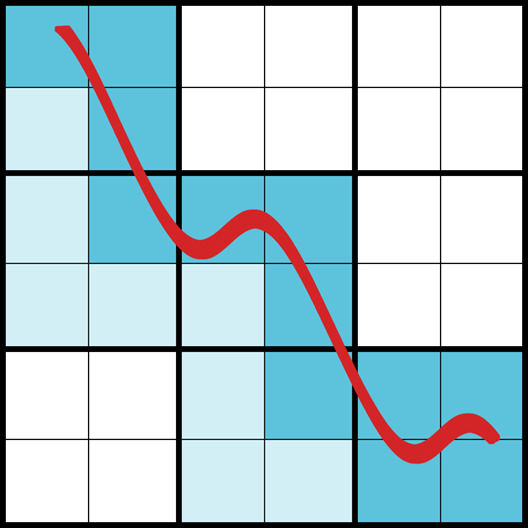
\includegraphics[height = .95\linewidth]{Images/line.png} \\ (a) simple line with box counting ratio of $\log_2\frac{12}{5} = 1.26$
                \end{minipage}
                \begin{minipage}{0.49\linewidth}
                        \small
                        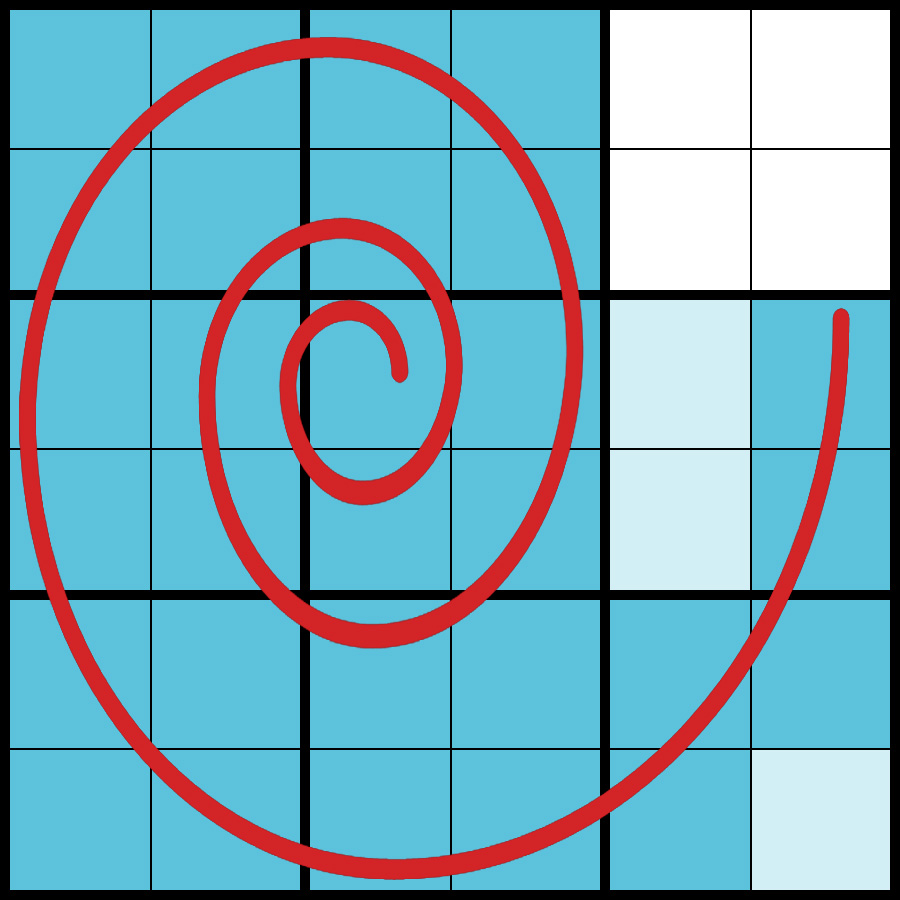
\includegraphics[height = .95\linewidth]{Images/spiral.jpg} \\ (b) complex line with box counting ratio of $\log_2\frac{29}{8} = 1.86$
                \end{minipage}
        \caption{Example of box counting ratio calculations on streamlines.}
        \label{fig:box_counting_calcs}
\end{figure}

\section{Streamline Complexity Grid} \label{sec:scg}

For each regular point $p$ in a vector field $f: \Rthree \Rightarrow \Rthree$,
let $\zeta_p$ be the unique streamline passing through $p$.
Define $\phi_w(p)$ as the local box counting ratio of $\zeta_p$
in a $\gDim{w}$ region around $p$,
where boxes have edge lengths $l$ and $2l$.
Function $\phi_w$ defines a scalar field on the regular points of $f$.
The scalar $\phi_w(p)$ represents the complexity of a streamline through $p$ in a $\gDim{w}$ neighborhood of $p$.
We call the scalar field $\phi_w$, the streamline complexity field of $f$.

To compute the set of streamlines, we first seed a streamline from each voxel $v$ in our vector field $f$.
We then calculate the box counting dimensions of each of these streamlines using the previously described box counting dimension algorithm.
If the streamline intersects more than a predefined cutoff of $c_s$ boxes of edge length $2l$, then the streamline is stored.
If the streamline does not intersect more than $c_s$ boxes, it is discarded.

To compute the local box counting ratio of $\zeta_v$ in a $\gDim{w}$ region centered at $v$, we take a subset of the streamline, $\zeta_s$, that precisely included in the portion of $\zeta_v$ that is within the $\gDim{w}$ region.
The box counting dimension of $\zeta_s$ is then computed using the previously described box counting dimension algorithm.
Similarly to the streamline generation step, it is also ensured that $\zeta_s$ intersects more than $c_v$ boxes of edge length $2l$.
If $\zeta_s$ does meet the cutoff requirement, the box counting dimension is considered a value estimate, if not, the value is discarded.

To construct a scalar grid representing the streamline complex field of $f$, a set of streamlines are generated as previously described.
For each streamline $\zeta_v$ that intersects voxel $v$, we compute the local box counting dimension of $\zeta_v$.
If $\zeta_v$ meets the cutoff requirement, the resulting box counting dimension is stored in a list with all other box counting dimensions calculated for $v$.
Once the local box counting dimension of all of the streamlines that intersect $v$ have been calculated, we take the $P$\textsuperscript{th} percentile of the local box counting dimension list and store this value as $v$'s complexity value.
Let the streamline whose local box counting dimension was measured as the $P$\textsuperscript{th} percentile local box counting dimension for voxel $v$ be denoted as $v_\zeta$.
We call the resulting scalar grid, the streamline complexity grid of $f$.

Additionally, a scalar value is associated with each streamline representing the streamline's complexity.
For a single streamline $\zeta_v$, its local box counting dimension is measured at each voxel that it intersects.
The highest of these local box counting dimension calculations is stored as the complexity value of $\zeta_v$ .

For clarity, a flow chart of a summarized version of the algorithm steps are displayed in Fig. \ref{fig:algorithm_flowchart}.

\begin{figure}
\begin{tikzpicture}[node distance = 2cm, auto]
    % Place nodes
    \node [block] (step1) {Generate a set of streamlines from each voxel.};
    \node [decision, below of=step1] (moreblocks) at (0,0) {Are there voxels with complexity values not set?};
    \node [block, right of=moreblocks, node distance=3cm] (end) {end};
    \node [block, below of=moreblocks, node distance=5cm] (step2) {\begin{varwidth}{15em}
    For the current voxel:
    \\$\bullet$find the list of streamlines that intersect the voxel
    \\$\bullet$compute the local box counting dimension for each streamline
    \\$\bullet$take the $P$\textsuperscript{th} percentile local box counting dimension and assign the voxel this value
    \end{varwidth}};
    % Draw edges
    \path [line] (step1) -- (moreblocks);
    \path [line] (moreblocks) -- node {no}(end);
    \path [line] (moreblocks) -- node {yes} (step2);
    \path [line] (step2) - ++(-3.5, 0) |- (moreblocks);
\end{tikzpicture}
    \caption{Flow chart of how the streamline complexity grid is generated.}
    \label{fig:algorithm_flowchart}
\end{figure}

\section{Visualization Techniques} \label{sec:vt}

The streamline complexity computations can be used in a variety of ways to filter streamlines of varying complexities or to provide a method of visualization for the flow field.

\subsection{Streamline filtering by value}
The user is able to choose two values, $a$ and $b$ where $a < b$, and only display streamlines with a complexity inbetween the chosen values. 
Specifically, the streamline $\zeta_p$ will be displayed only if $a \leq \phi_w(p) \leq b$.
The constants allow the user to choose the level of streamline complexity that they will view.
By choosing constants of values near 1, streamlines with a low box counting ratio and smooth flow will be displayed.
By choosing constants of values above 2, streamlines with a relatively high box counting ratio and turbulent or complex flow will be displayed.
Filtering by complexity value is shown in Fig. \ref{fig:value_filter}

\begin{figure}[h]
        \centering
                \begin{minipage}{0.30\linewidth}
               		\small
                       	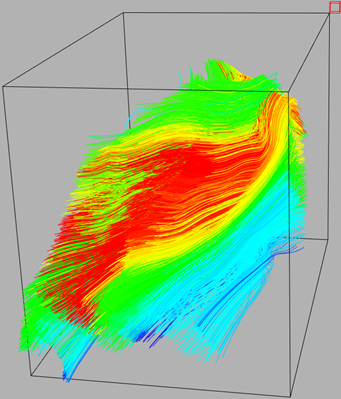
\includegraphics[height = 1.1\linewidth]{Images/all_vtk.png}\\(a) the cluttered view of all of the streamlines in the dataset\vspace{0.2em}
                \end{minipage}
                \begin{minipage}{0.30\linewidth}
                	\small
                        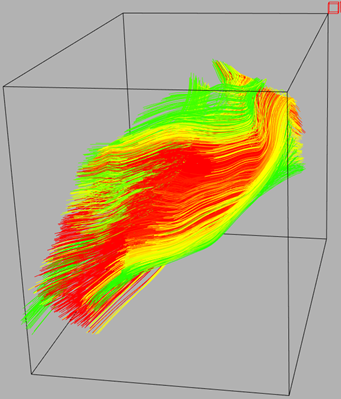
\includegraphics[height = 1.1\linewidth]{Images/filter_vtk.png}\\(b) the filtered streamlines above a certain complexity value \vspace{0.2em}
                \end{minipage}
                \begin{minipage}{0.30\linewidth}
                	\small
                        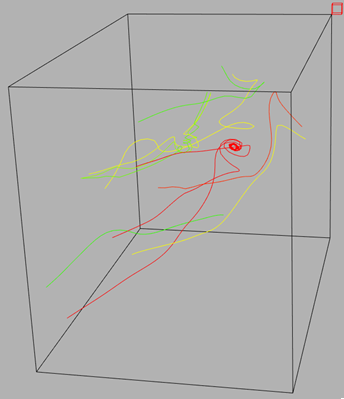
\includegraphics[height = 1.1\linewidth]{Images/max_vtk.png}\\(c) the filtered streamlines above only at local maximums \vspace{0.2em}
                \end{minipage}
        \caption{Example of the streamline filtering techniques.}
        \label{fig:value_filter}
\end{figure}

\subsection{Local complexity maximums}
A significant amount of clutter in the streamline display will remain if additional filtering methods are not considered.
Several streamlines in the visualization will be visually similar or provide redundant information.
We are able to only show the local maximum streamlines to filter streamlines that all represent a single region or feature of the flow.
Local maximum filtering will show streamline $v_\zeta$ only if for all of the 8 points $q$ that directly neighbor $v$ on the complexity grid, $\phi_w(v) > \phi_w(q)$.
This method allows for single streamlines representatives to be shown for each feature or region rather than several, cluttered streamlines.

\subsection{Colored plane}
A colored plane can be used to allow the user to visualize the scalar complexity grid, $\phi_p$, directly.
A color gradient from blue to green to red is able to be defined and mapped to values in the range 0 to 3, for each of the possible box counting dimensions ratios.
Low scalar values will be displayed as blue colors, while high scalar values will be displayed as red colors.
A plane is then defined on the scalar complexity grid and each point on the plane is colored from this defined color gradient.
The user is able to control the plane through the scalar complexity grid to identfiy regions varying complexity in the grid.
Once regions of interest are identified through the color plane, the user can display streamlines near that region to understand its behavior.

\subsection{Complexity samplings}
The streamlines seeded from the region of the colored plane can be viewed in various samplings to show the different levels of complexity around the plane.
The scalar values on the colored planes are partitioned into two sets, the one-third highest scalar values and the two-thirds lowest scalar values.
Two sets of streamlines are also constructed.
For the voxels that the plane intersects, $S_{top} = \{ v_\zeta | \phi_w(v)$ is in the top one-third scalar values$\}$ and $S_{bottom} = \{ v_\zeta | \phi_w(v$) is in the bottom two-thirds scalar values $\}$.
Two values are then defined by the user to determine the percentages of $S_{top}$ and $S_{bottom}$ displayed.
An example of the plane visualizations are shown in Fig. \ref{fig:plane}.

\begin{figure}[h]
        \centering
                \begin{minipage}{0.45\linewidth}
                        \small
                        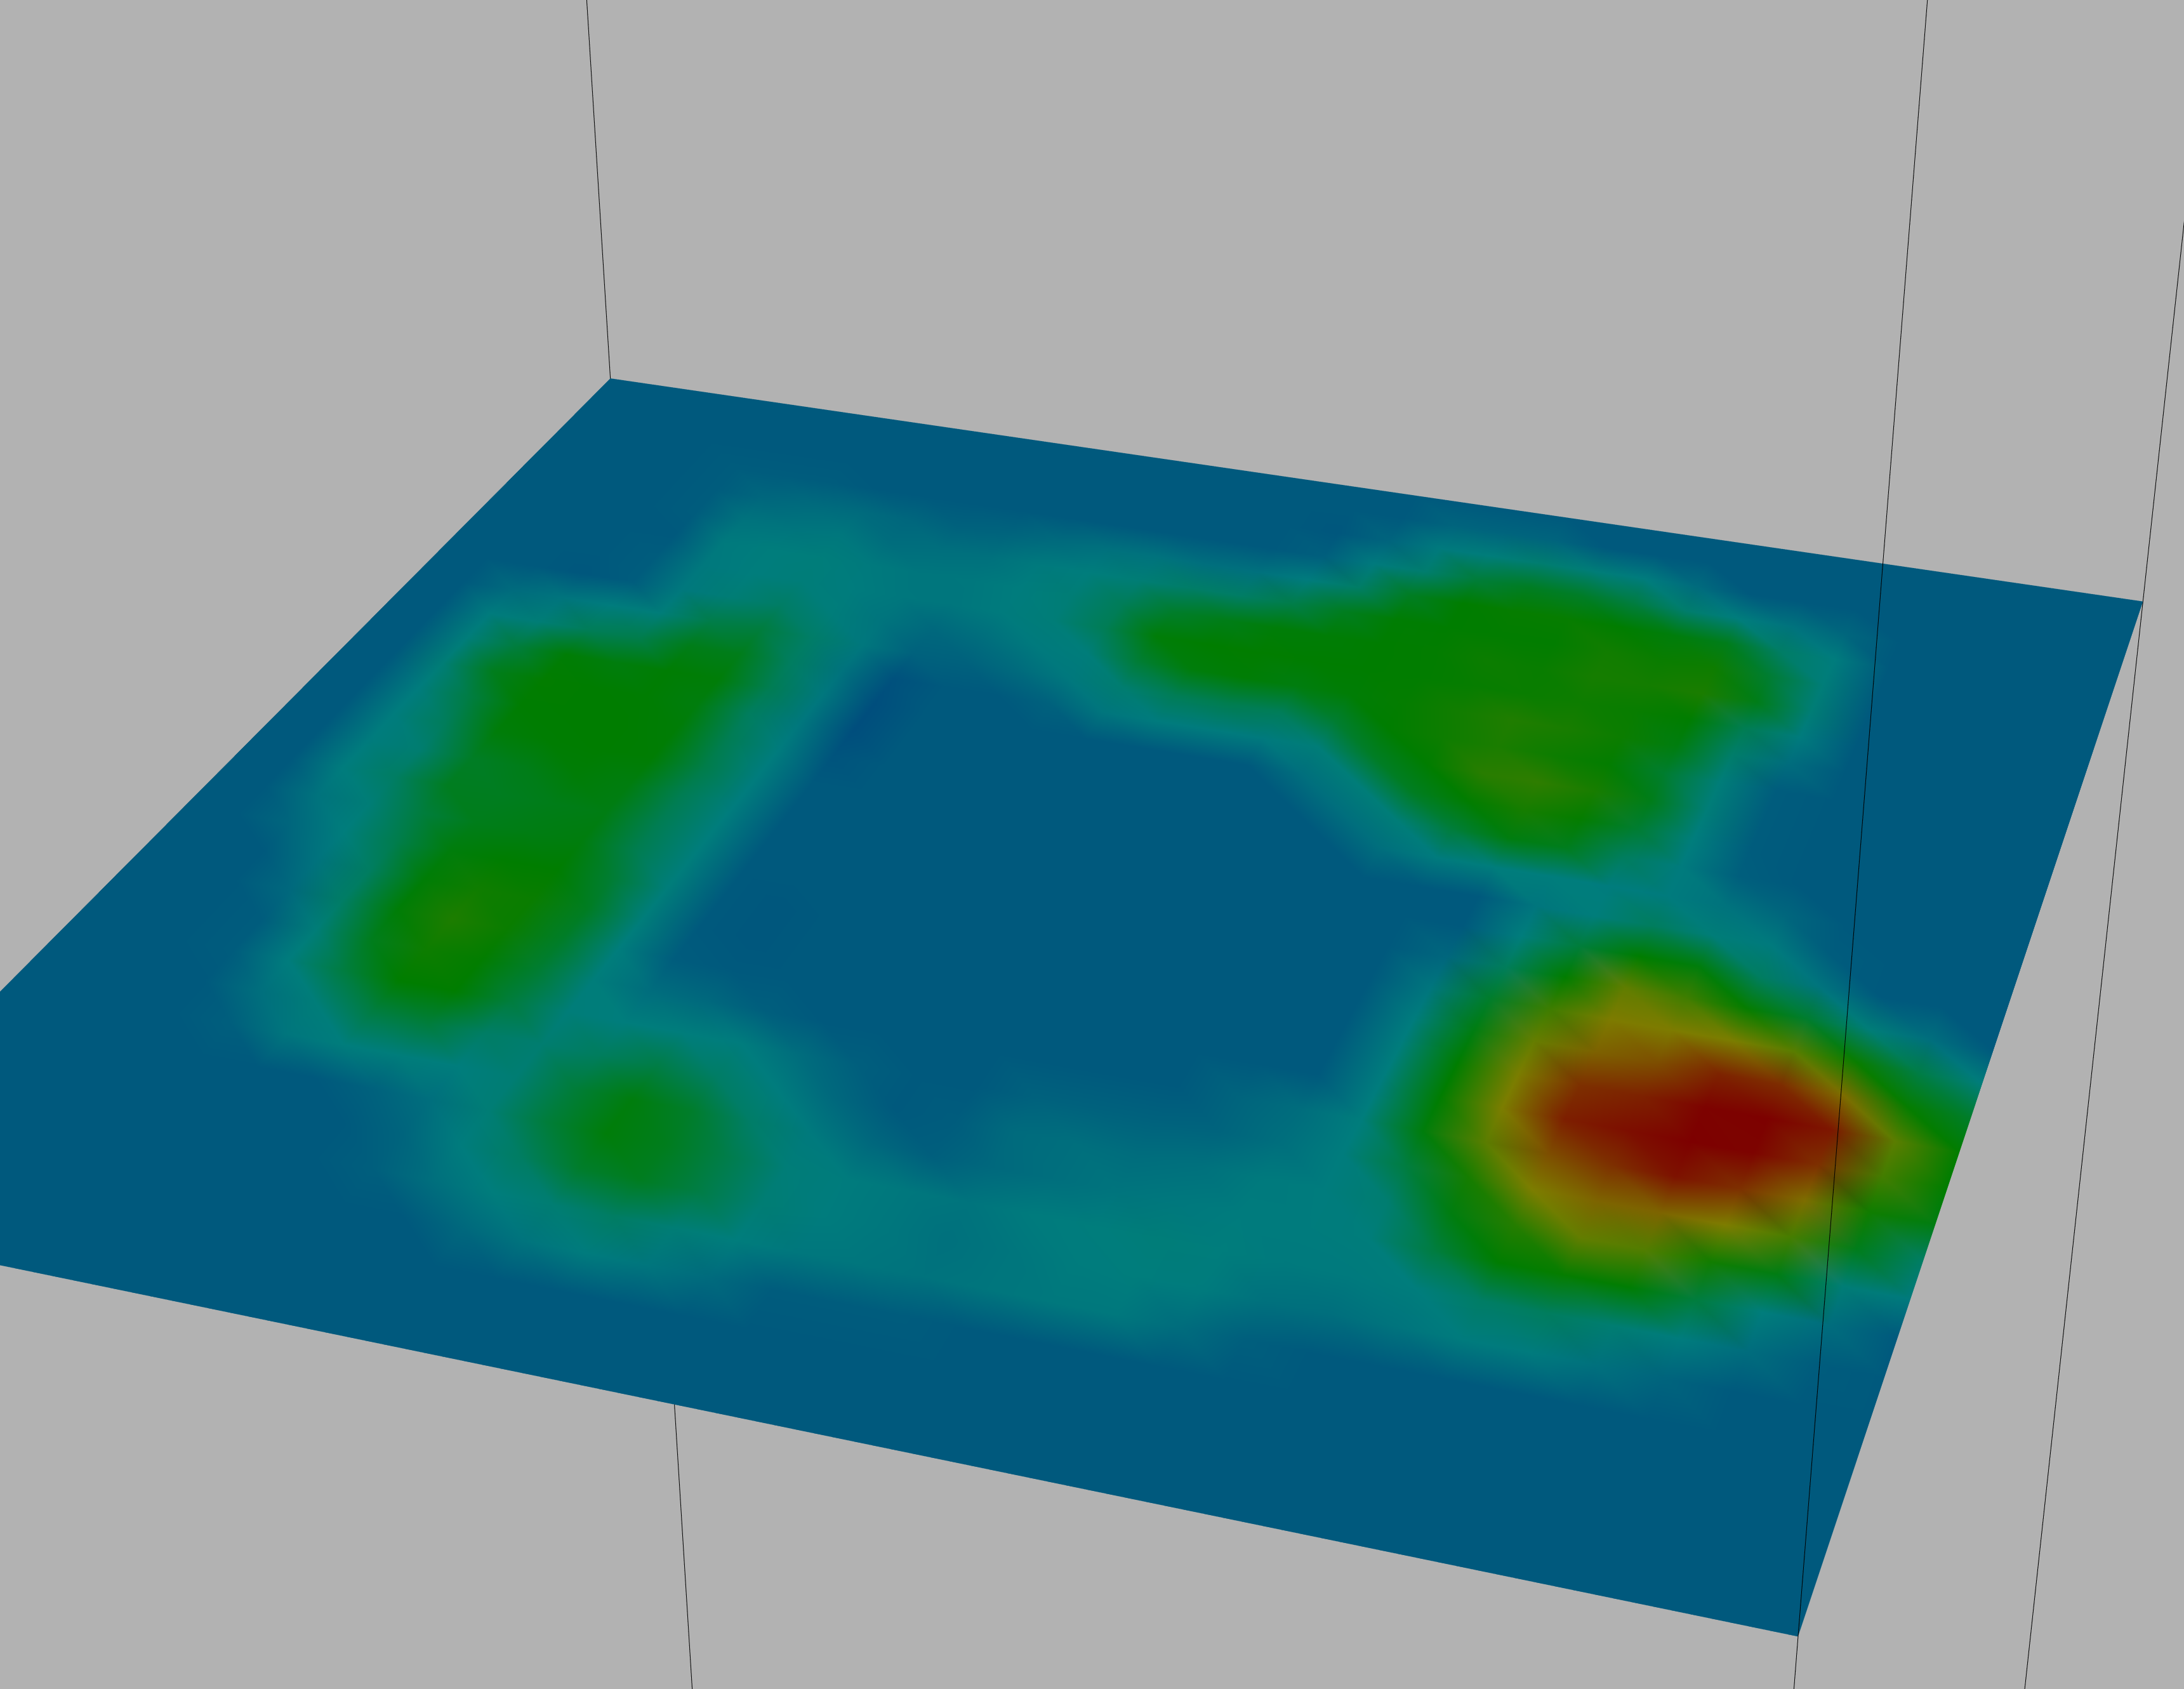
\includegraphics[height = 0.75\linewidth]{Images/plane_crop.png}\\(a) the plane indicating the regions of high complexity\vspace{0.2em}
                \end{minipage}
                \begin{minipage}{0.45\linewidth}
                        \small
                        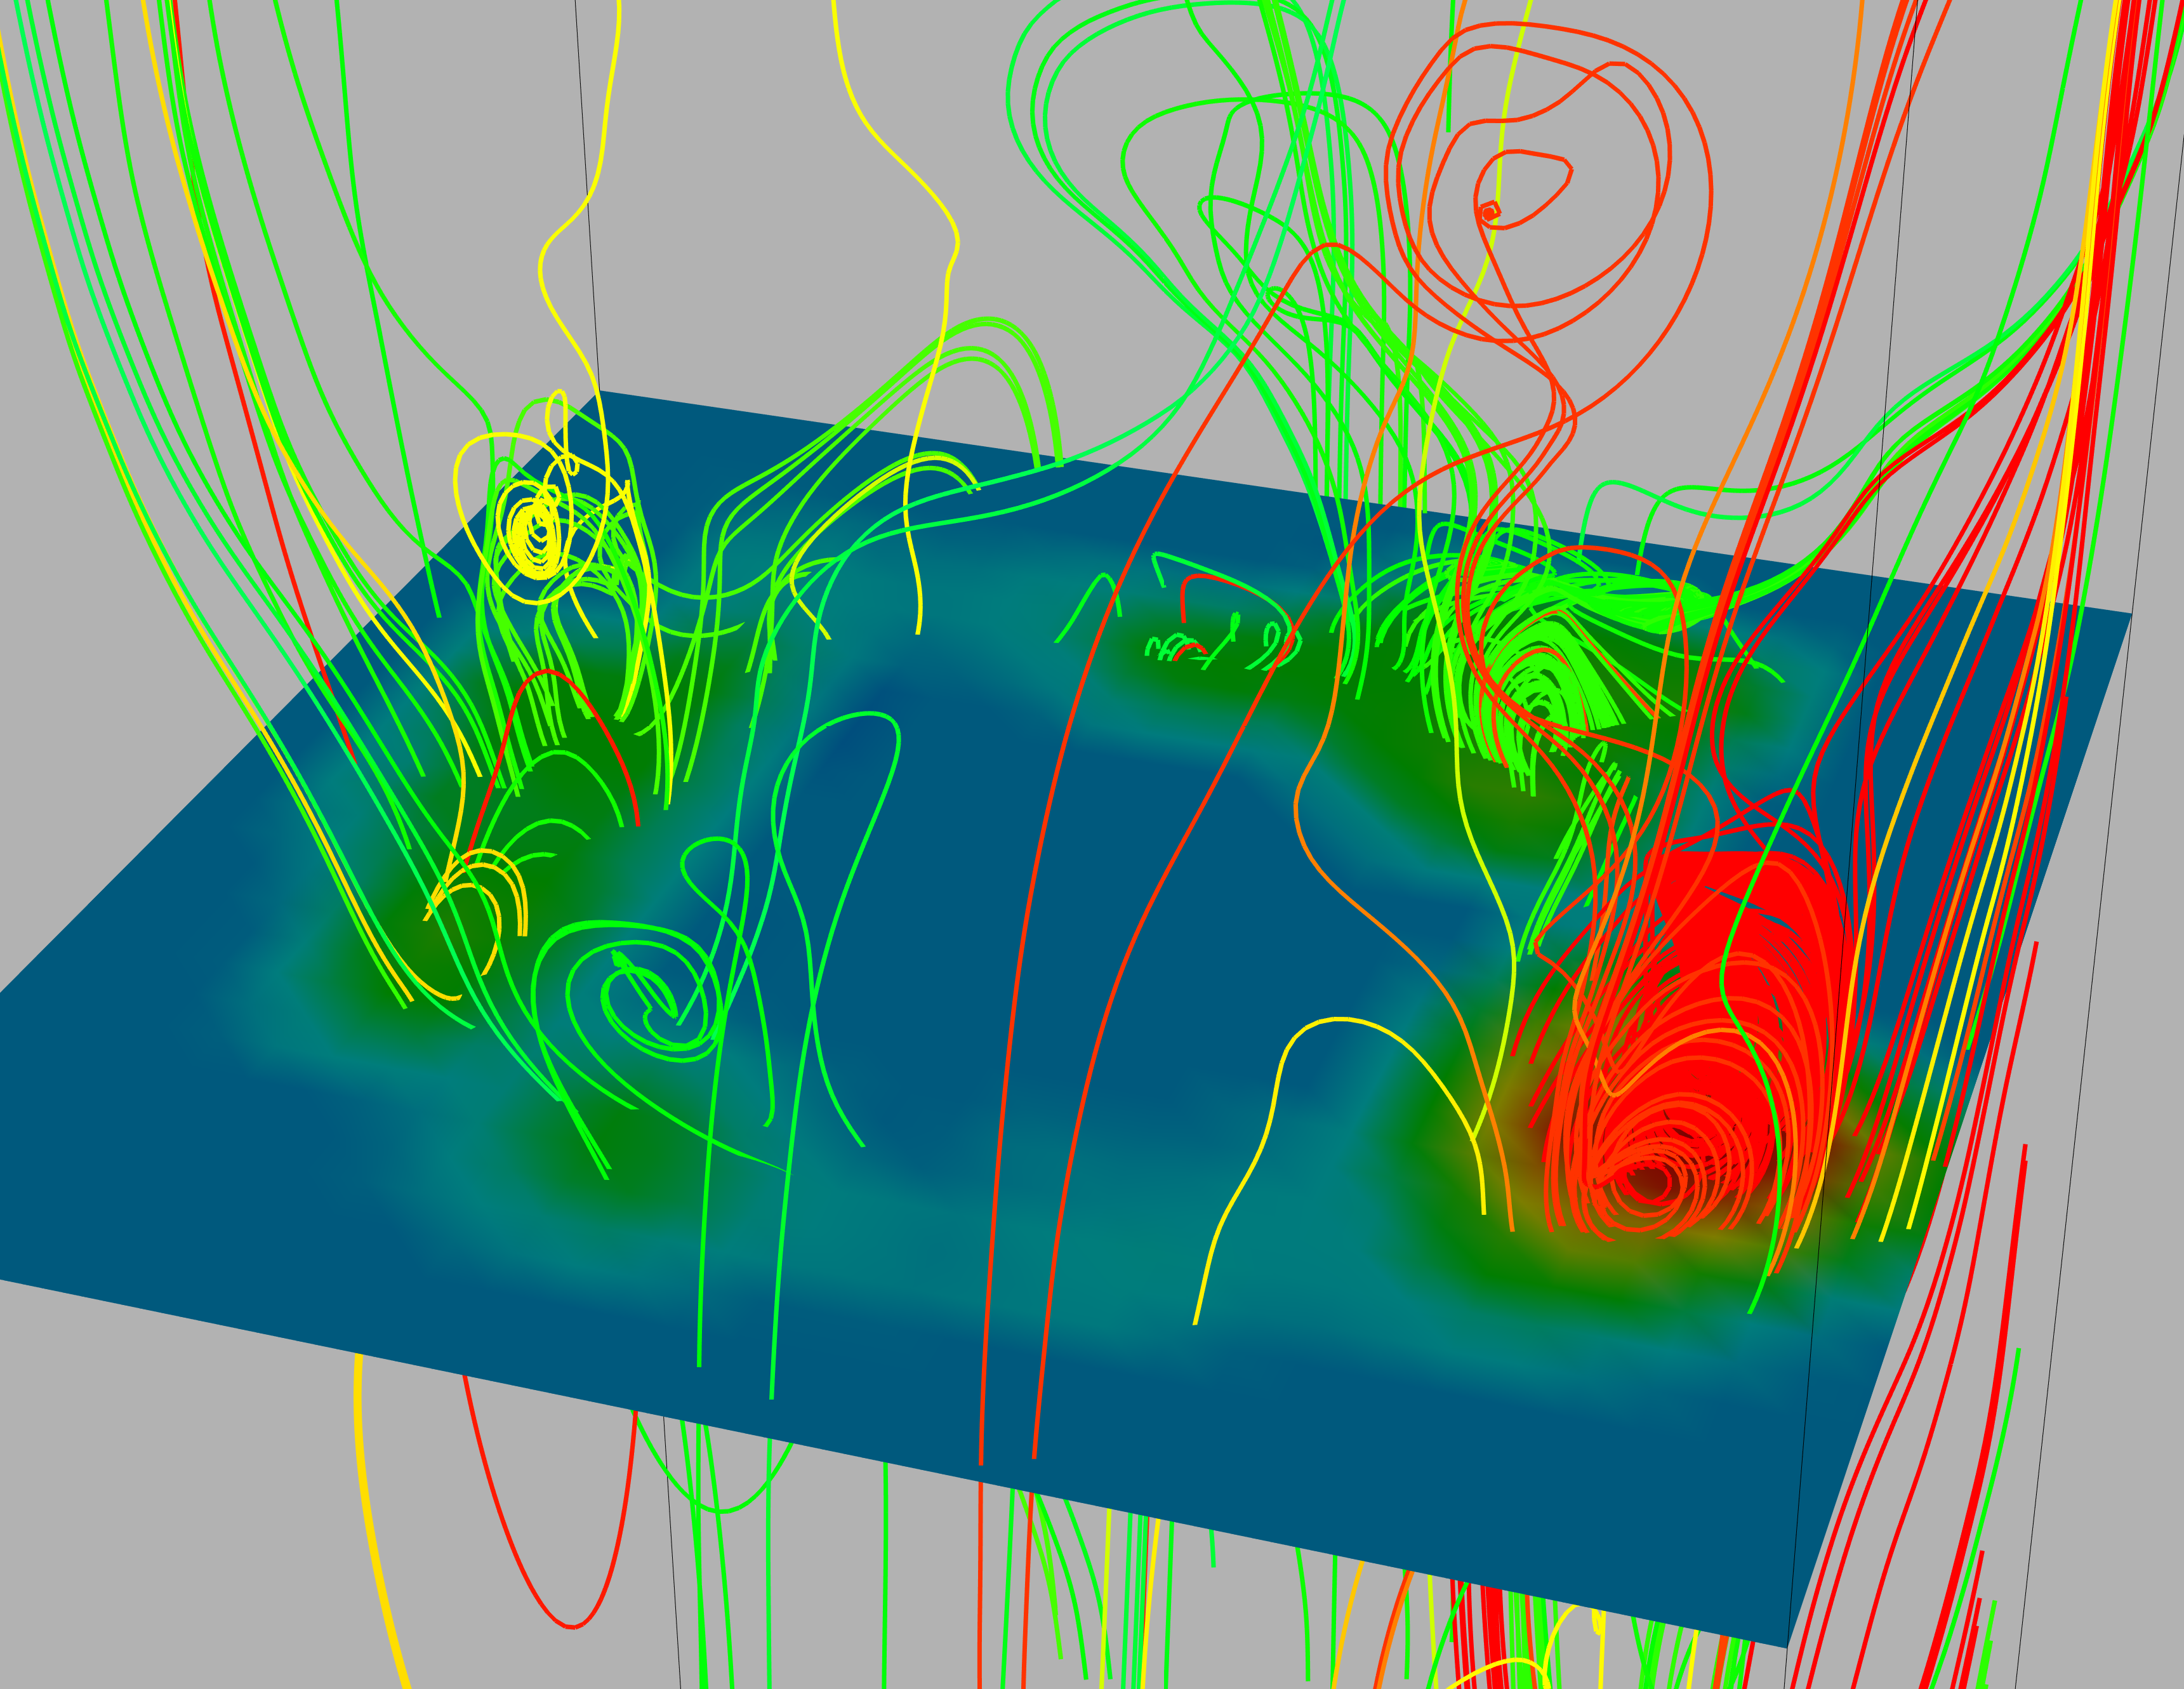
\includegraphics[height = 0.75\linewidth]{Images/plane_line_crop.png}\\(b) the high complexity lines near the defined plane.\vspace{0.2em}
                \end{minipage}
        \caption{Example visualizations using the colored plane.}
        \label{fig:plane}
\end{figure}

\subsection{Isosurfaces:} 
An isosurface can be used to highlight regions of the flow field with a high complexity.
An isosurface, which is defined by
\begin{equation} \{ x \mid \phi_w(x) = \sigma \}\end{equation}
where $\sigma$ is the isovalue and $\phi_w$ is the streamline complexity field, will seperate all scalar values above $\sigma$ from the values below $\sigma$ on the streamlines complexity.
This isosurface will enclose the regions of streamlines with a fractal dimension higher than the $\sigma$ value and provide a simple way to identify regions of a defined complexity.
At particularly high $\sigma$ values, the isosurface will only enclose vortices and turbulent features of the flow field that the user may have otherwise missed.

\subsection{Streamline gradient magnitudes:}
The gradient magnitudes of the streamline complexity grid can be calculated to create a new gradient magnitude scalar grid $\phi_g$.
The scalar $\phi_g(x)$ is given by $\| \nabla \phi_p(x) \|$.
Another isosurface can be used to visualization the function $\phi_g$ to identify regions of high change of turbulence or complexity.
Vortices in the flow field tend to have high complexity values recorded near their centers, with values quickly decreasing towards their boundaries.
When a high isovalue is chosen for the gradient magnitude isosurface's isovalue, the isosurface will highlight these isolated regions of turbulence or turbulent regions that quickly become smooth.
Example of isosurfaces of the scalar complexity values and gradient magnitudes are shown in Fig. \ref{fig:iso}.

\begin{figure}[h]
        \centering
                \begin{minipage}{0.47\linewidth}
                        \small
                        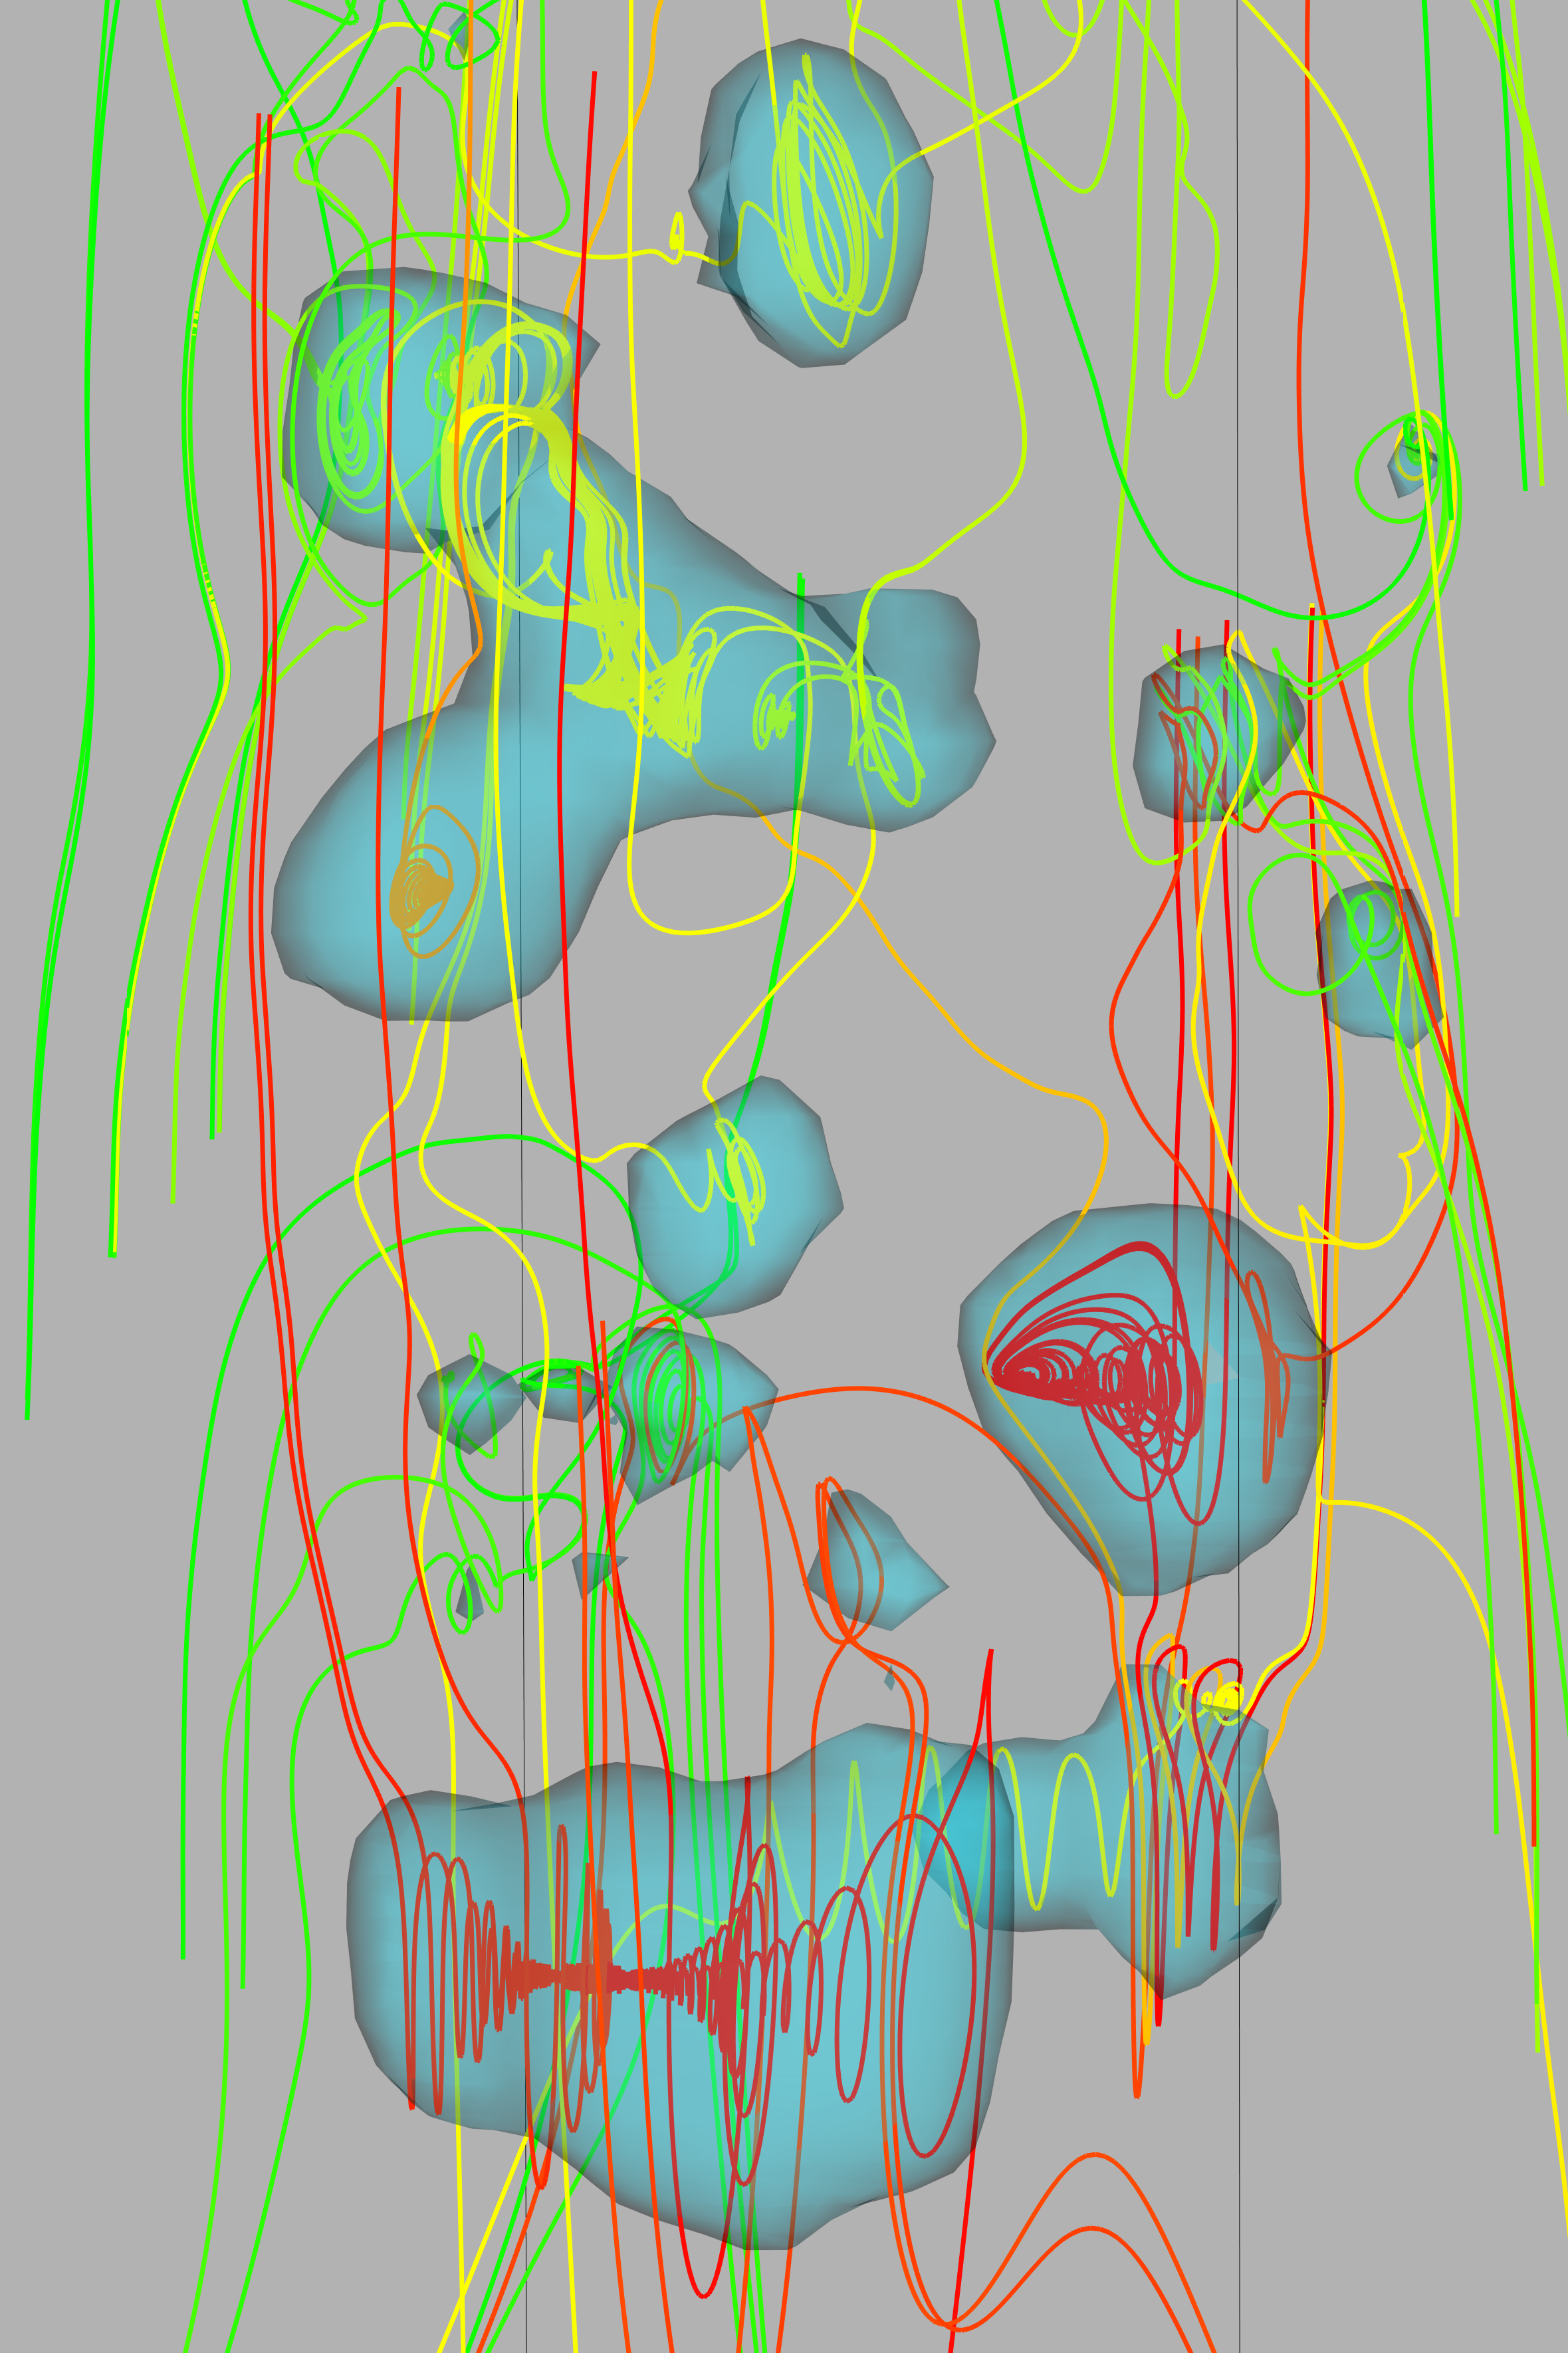
\includegraphics[height = 1.47\linewidth]{Images/iso_crop.png}\\(a) the scalar value isosurface enclosing high complexity regions\vspace{0.2em}
                \end{minipage}
                \begin{minipage}{0.47\linewidth}
                        \small
                        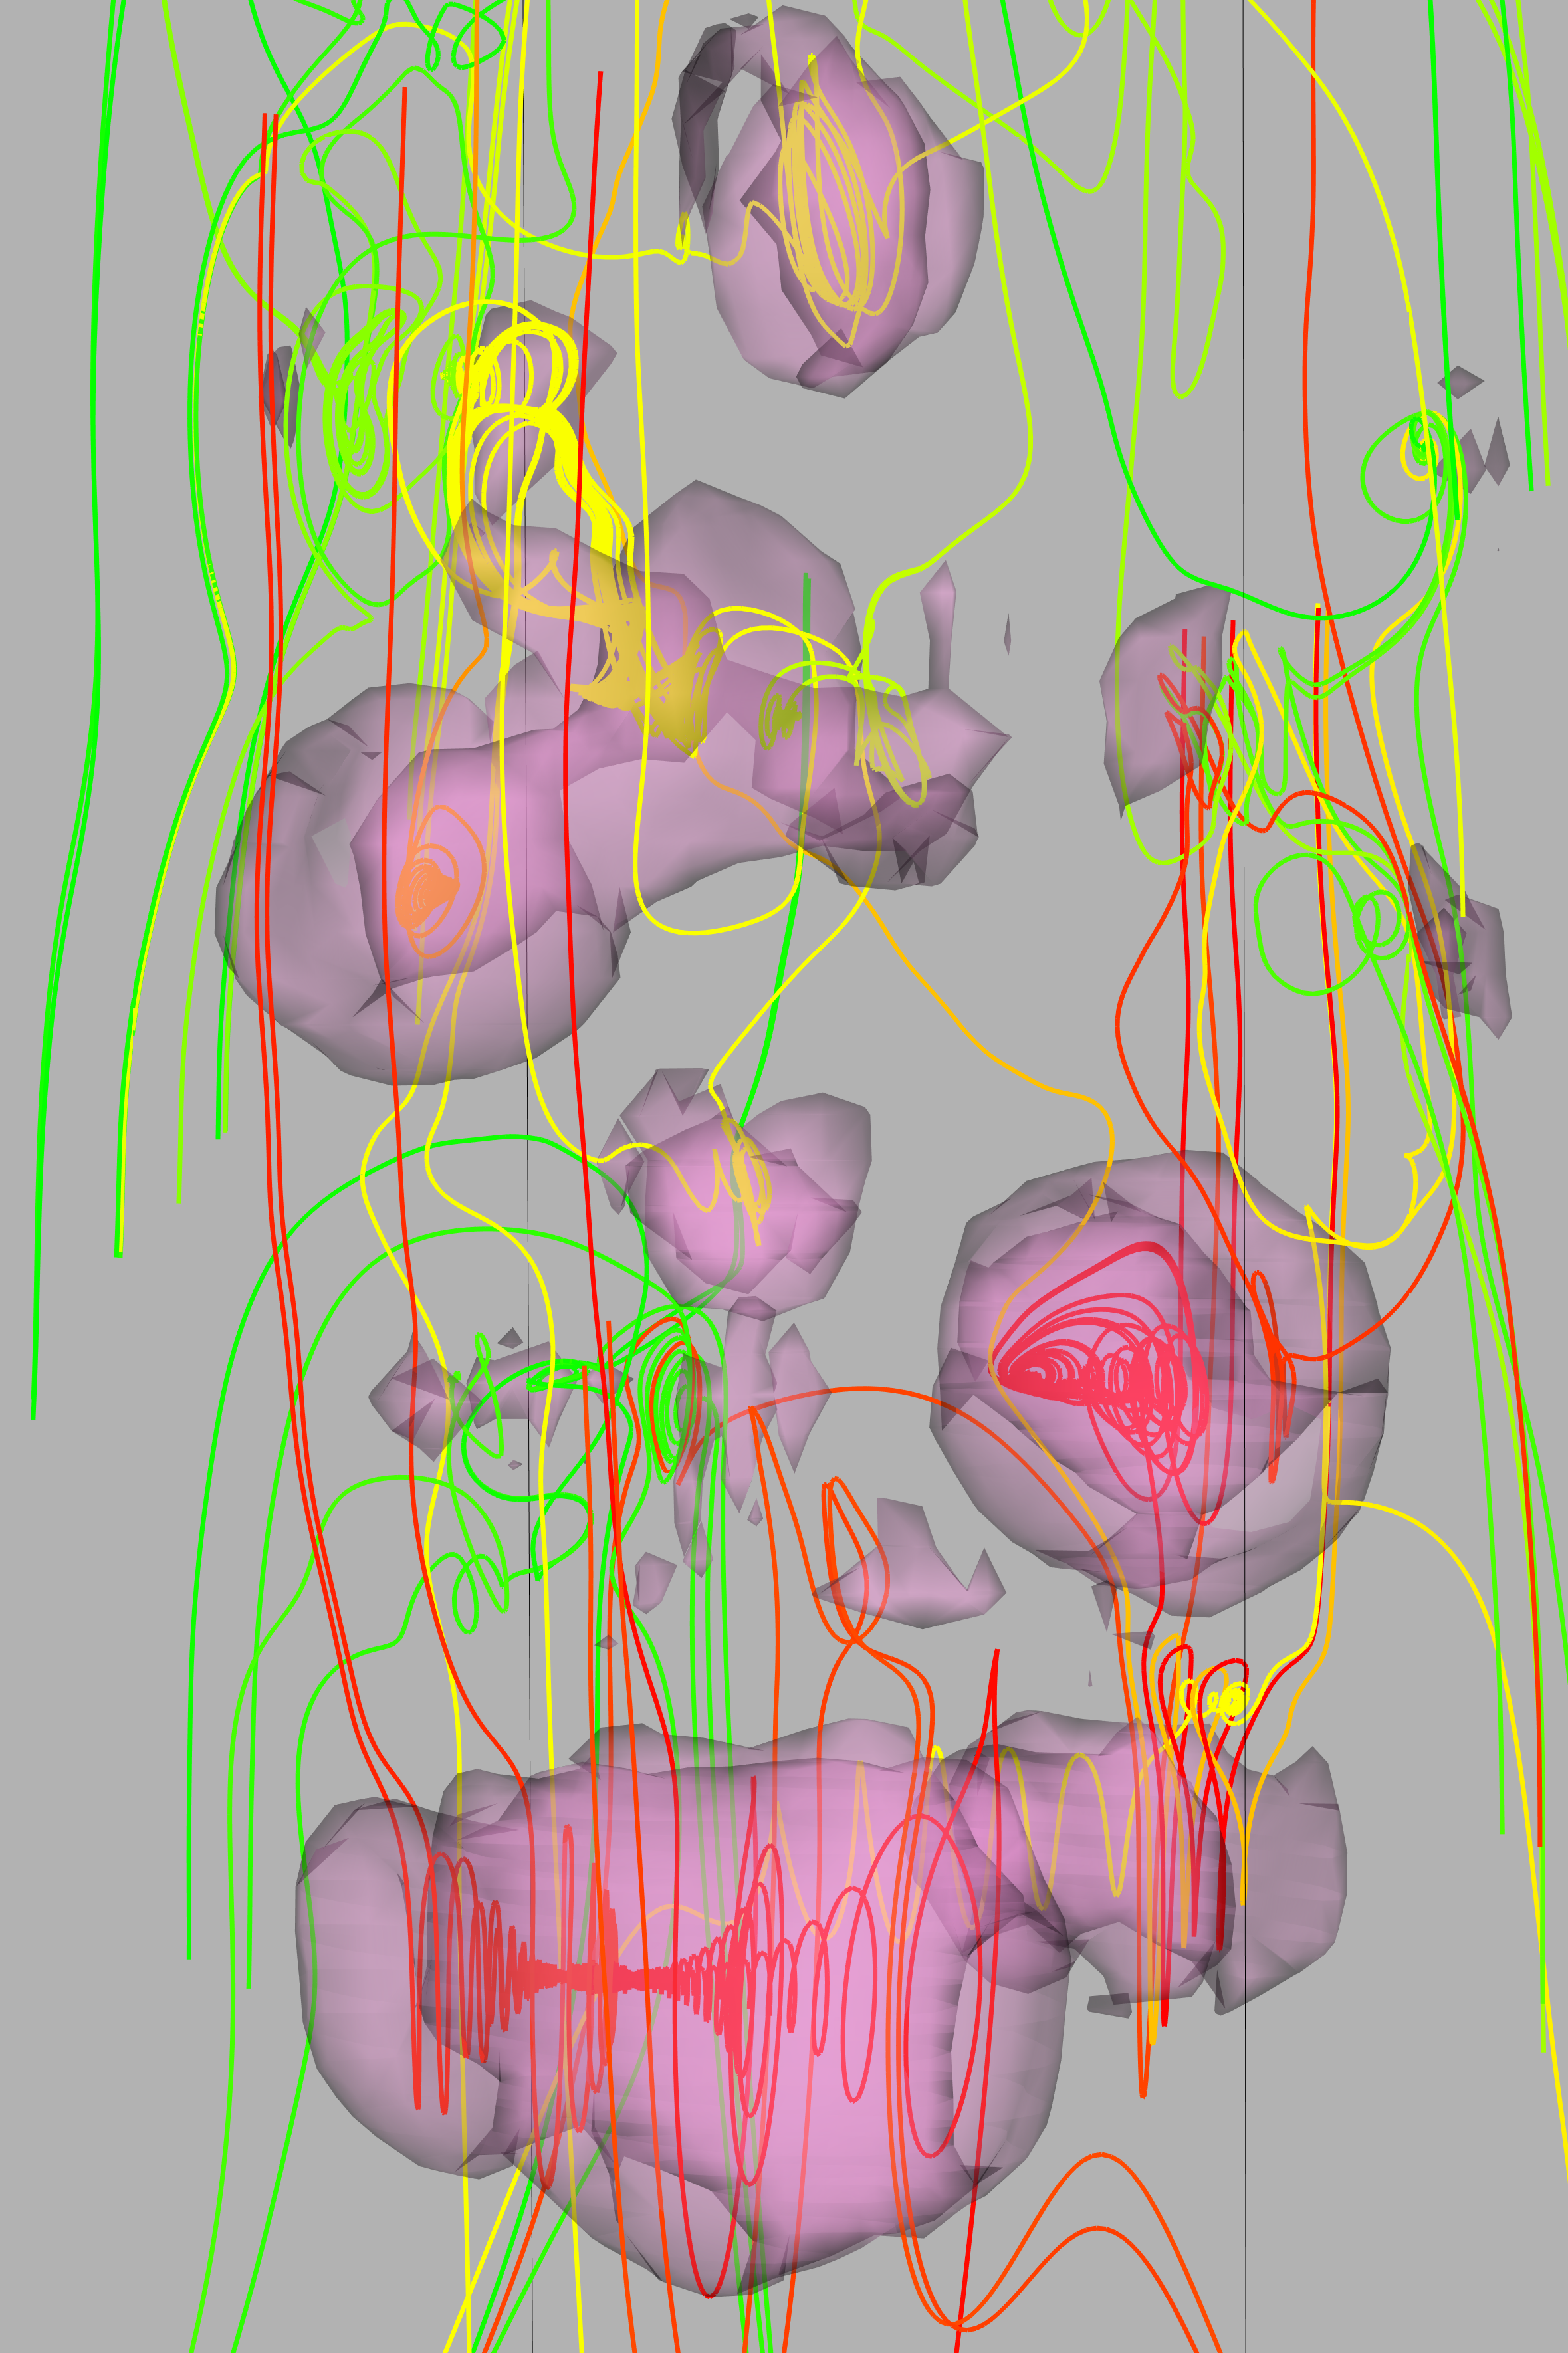
\includegraphics[height = 1.47\linewidth]{Images/grad_crop.png}\\(b) the gradient isosurface enclosing regions of high complexity change. \vspace{0.2em}
                \end{minipage}
        \caption{Example visualizations with isosurfaces.}
        \label{fig:iso}
\end{figure}

\section{Examples (or Results?)} \label{sec:examples}

In this section we will demonstrate how the previous described techiques can enhance the visualization of large flow field data sets.
The previously decribed algorithms and techniques are applied to two different data sets, a Solar Plume data set and a Hurricane Isabel data set.
Explanations and figures are given to show the advantages and features given by our algorithms.

The algorithm was implented in C++ using The Visualization Toolkit (VTK) across two seperate programs.
The first program has been created to generate streamlines, computer complexity measurements, and compute the streamline complexity grid and then output this information into files.
Then another program takes the output files as input and allows the user to interact with the streamlines and the streamline complexity grid.
The second program allows for a real-time interactivity with the flow data set.

\subsection{Solar Plume}

The Solar Plume data is a $126 \times 126 \times 512$ vector field data set that was provided by (who?).
This data set has many different regions of varying flow complexity.
Central regions of the flow tend to be more laminar with vortices near the boundaries of the data set.
These regions are able to be identified and highlighted by our algorithm.

A regular sampling of streamlines from the Solar Plume data set is displayed in Fig. \ref{fig:plume_lines}.a.
From the figure it is apparent that due to the size of this data set that a regular sampling is not suitable for this data set.
The streamlines cause severe occlusion and none of the strucutre of the flow field can be understood.
A filtering of the streamlines produced by considering the complexity measurements of the streamline given by our algorithm is displayed in Fig. \ref{fig:plume_lines}.b.
The filtering drastically reduces the clutter in the visualization and makes the regions of interest much more clear to the user.
To filter the streamlines in the plume data set, we are using the local maximum filtering as well as only showing the streamlines above a complexity value near 1.6.
The streamlines are also colored by complexity, with the red streamlines being the most complex and oftern contain vortices.
The green and less complex streamlines only contain mild turbulence through the line.
The isosurface is in this rendering is set to a value near 1.6 to enclose the complex regions of the line.

\begin{figure}[h]
        \centering
                \begin{minipage}{0.47\linewidth}
                       %% \centering \small
                        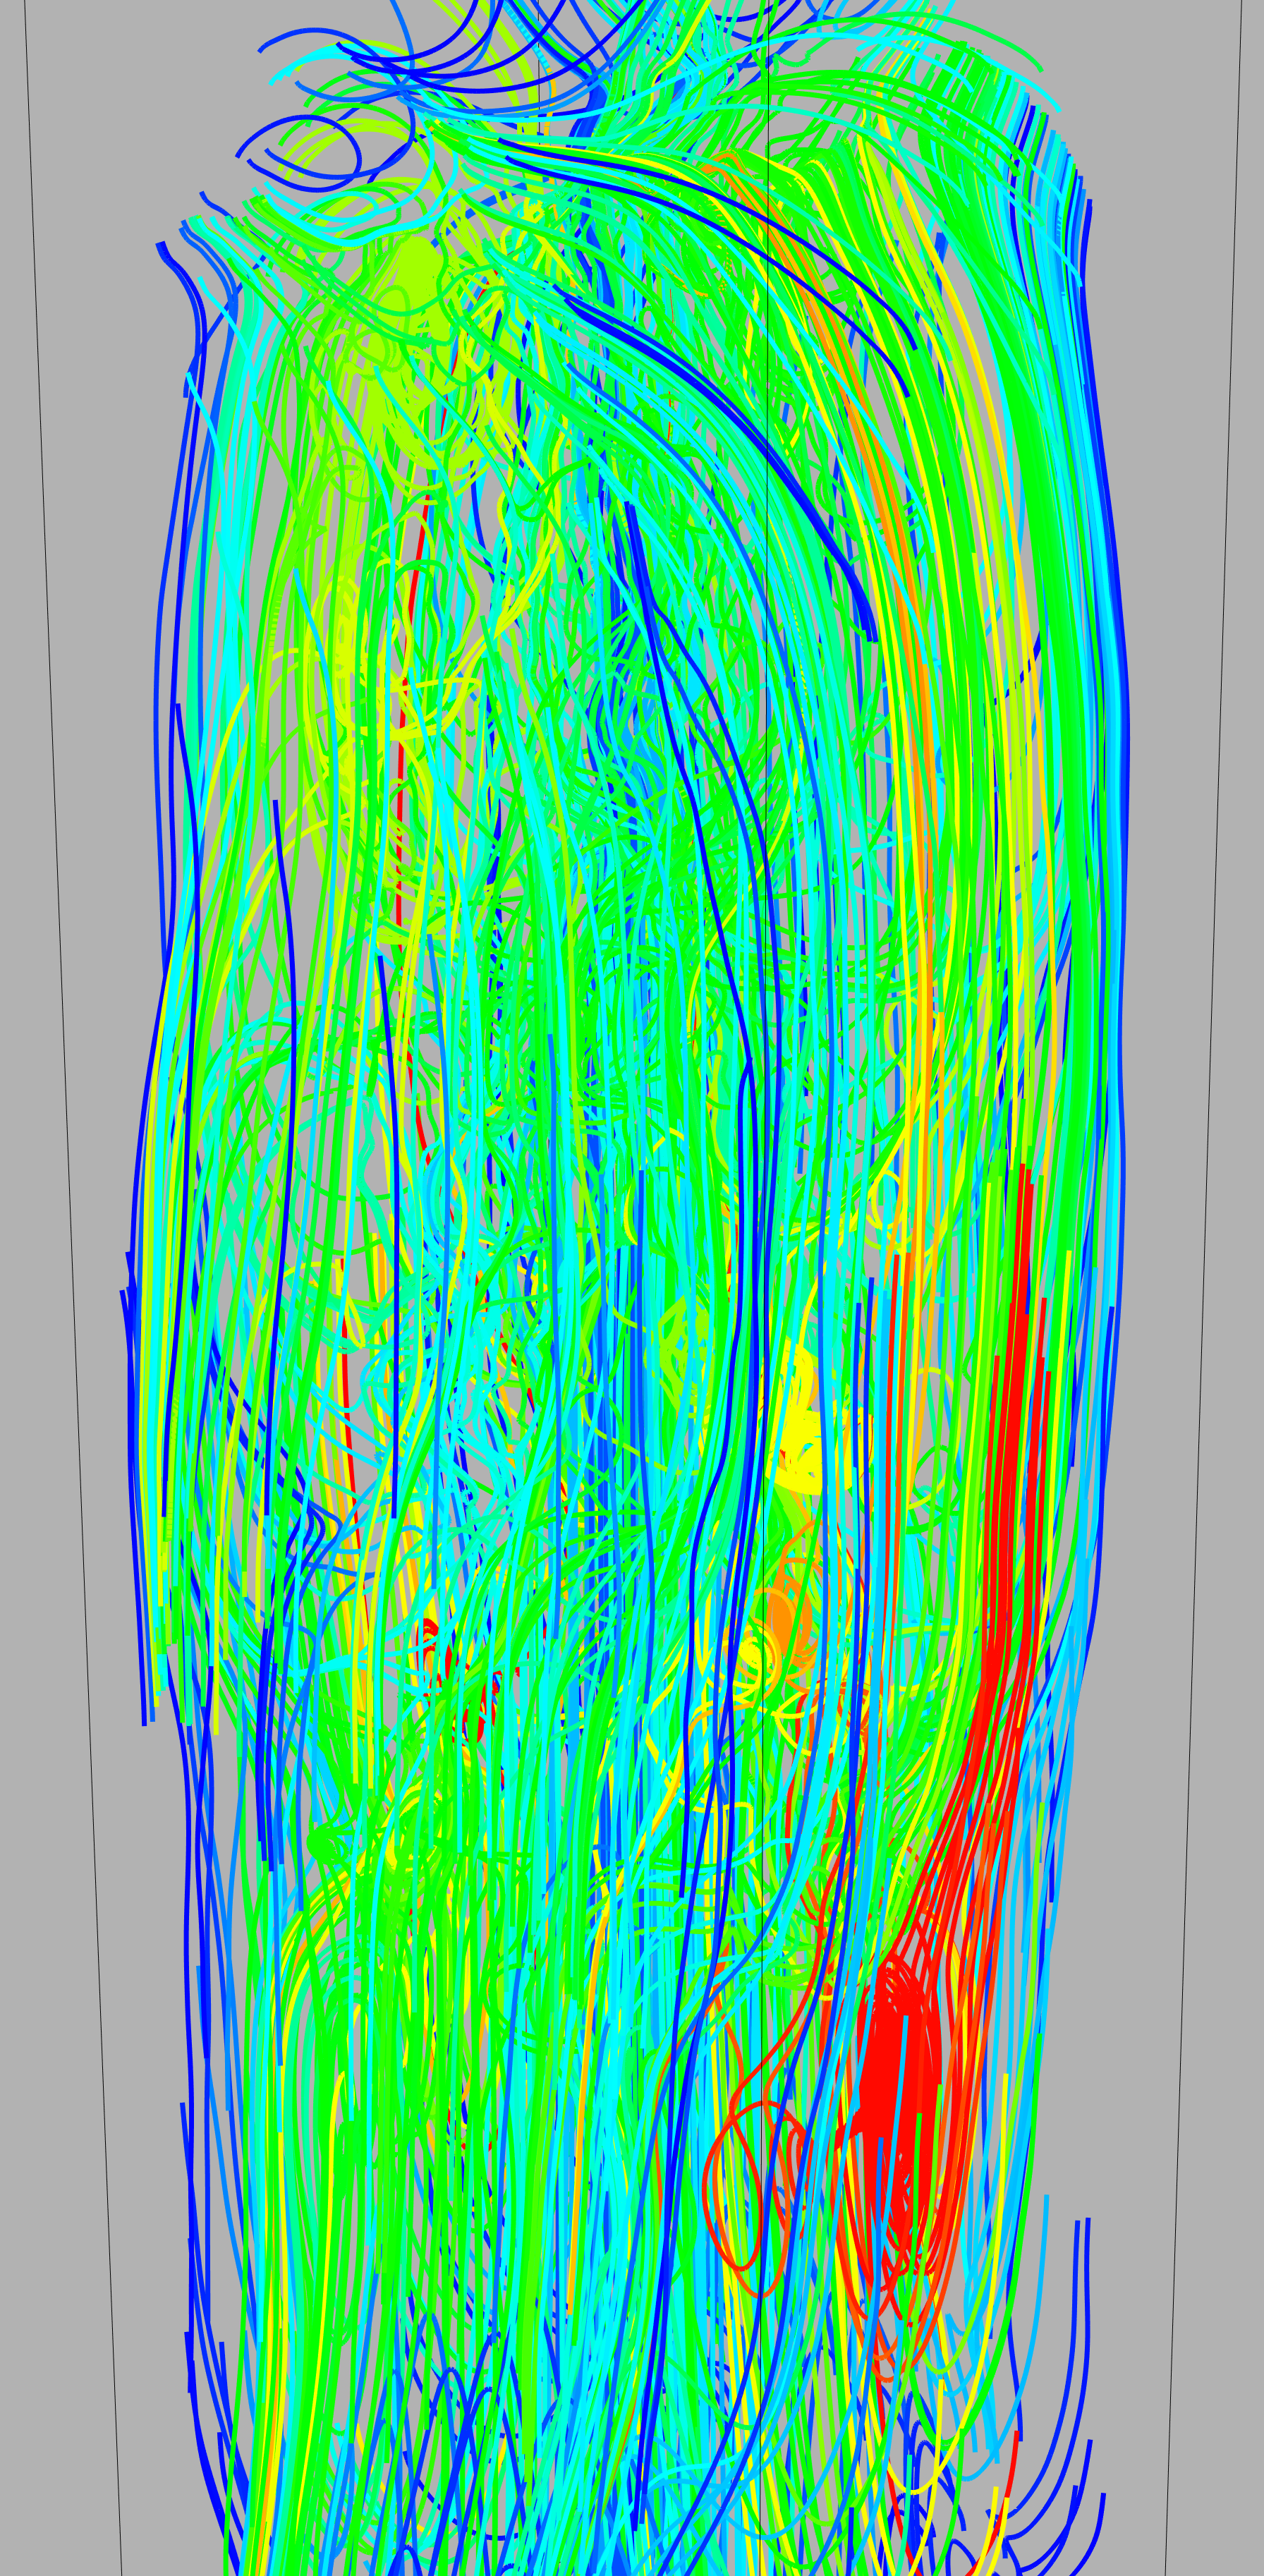
\includegraphics[height = 2\linewidth]{Images/plume_all_crop.png}\\(a) Streamlines seeded regularly through the Solar Plume data set. \vspace{0.2em}
                \end{minipage}
                \begin{minipage}{0.47\linewidth}
                       %% \centering \small
                        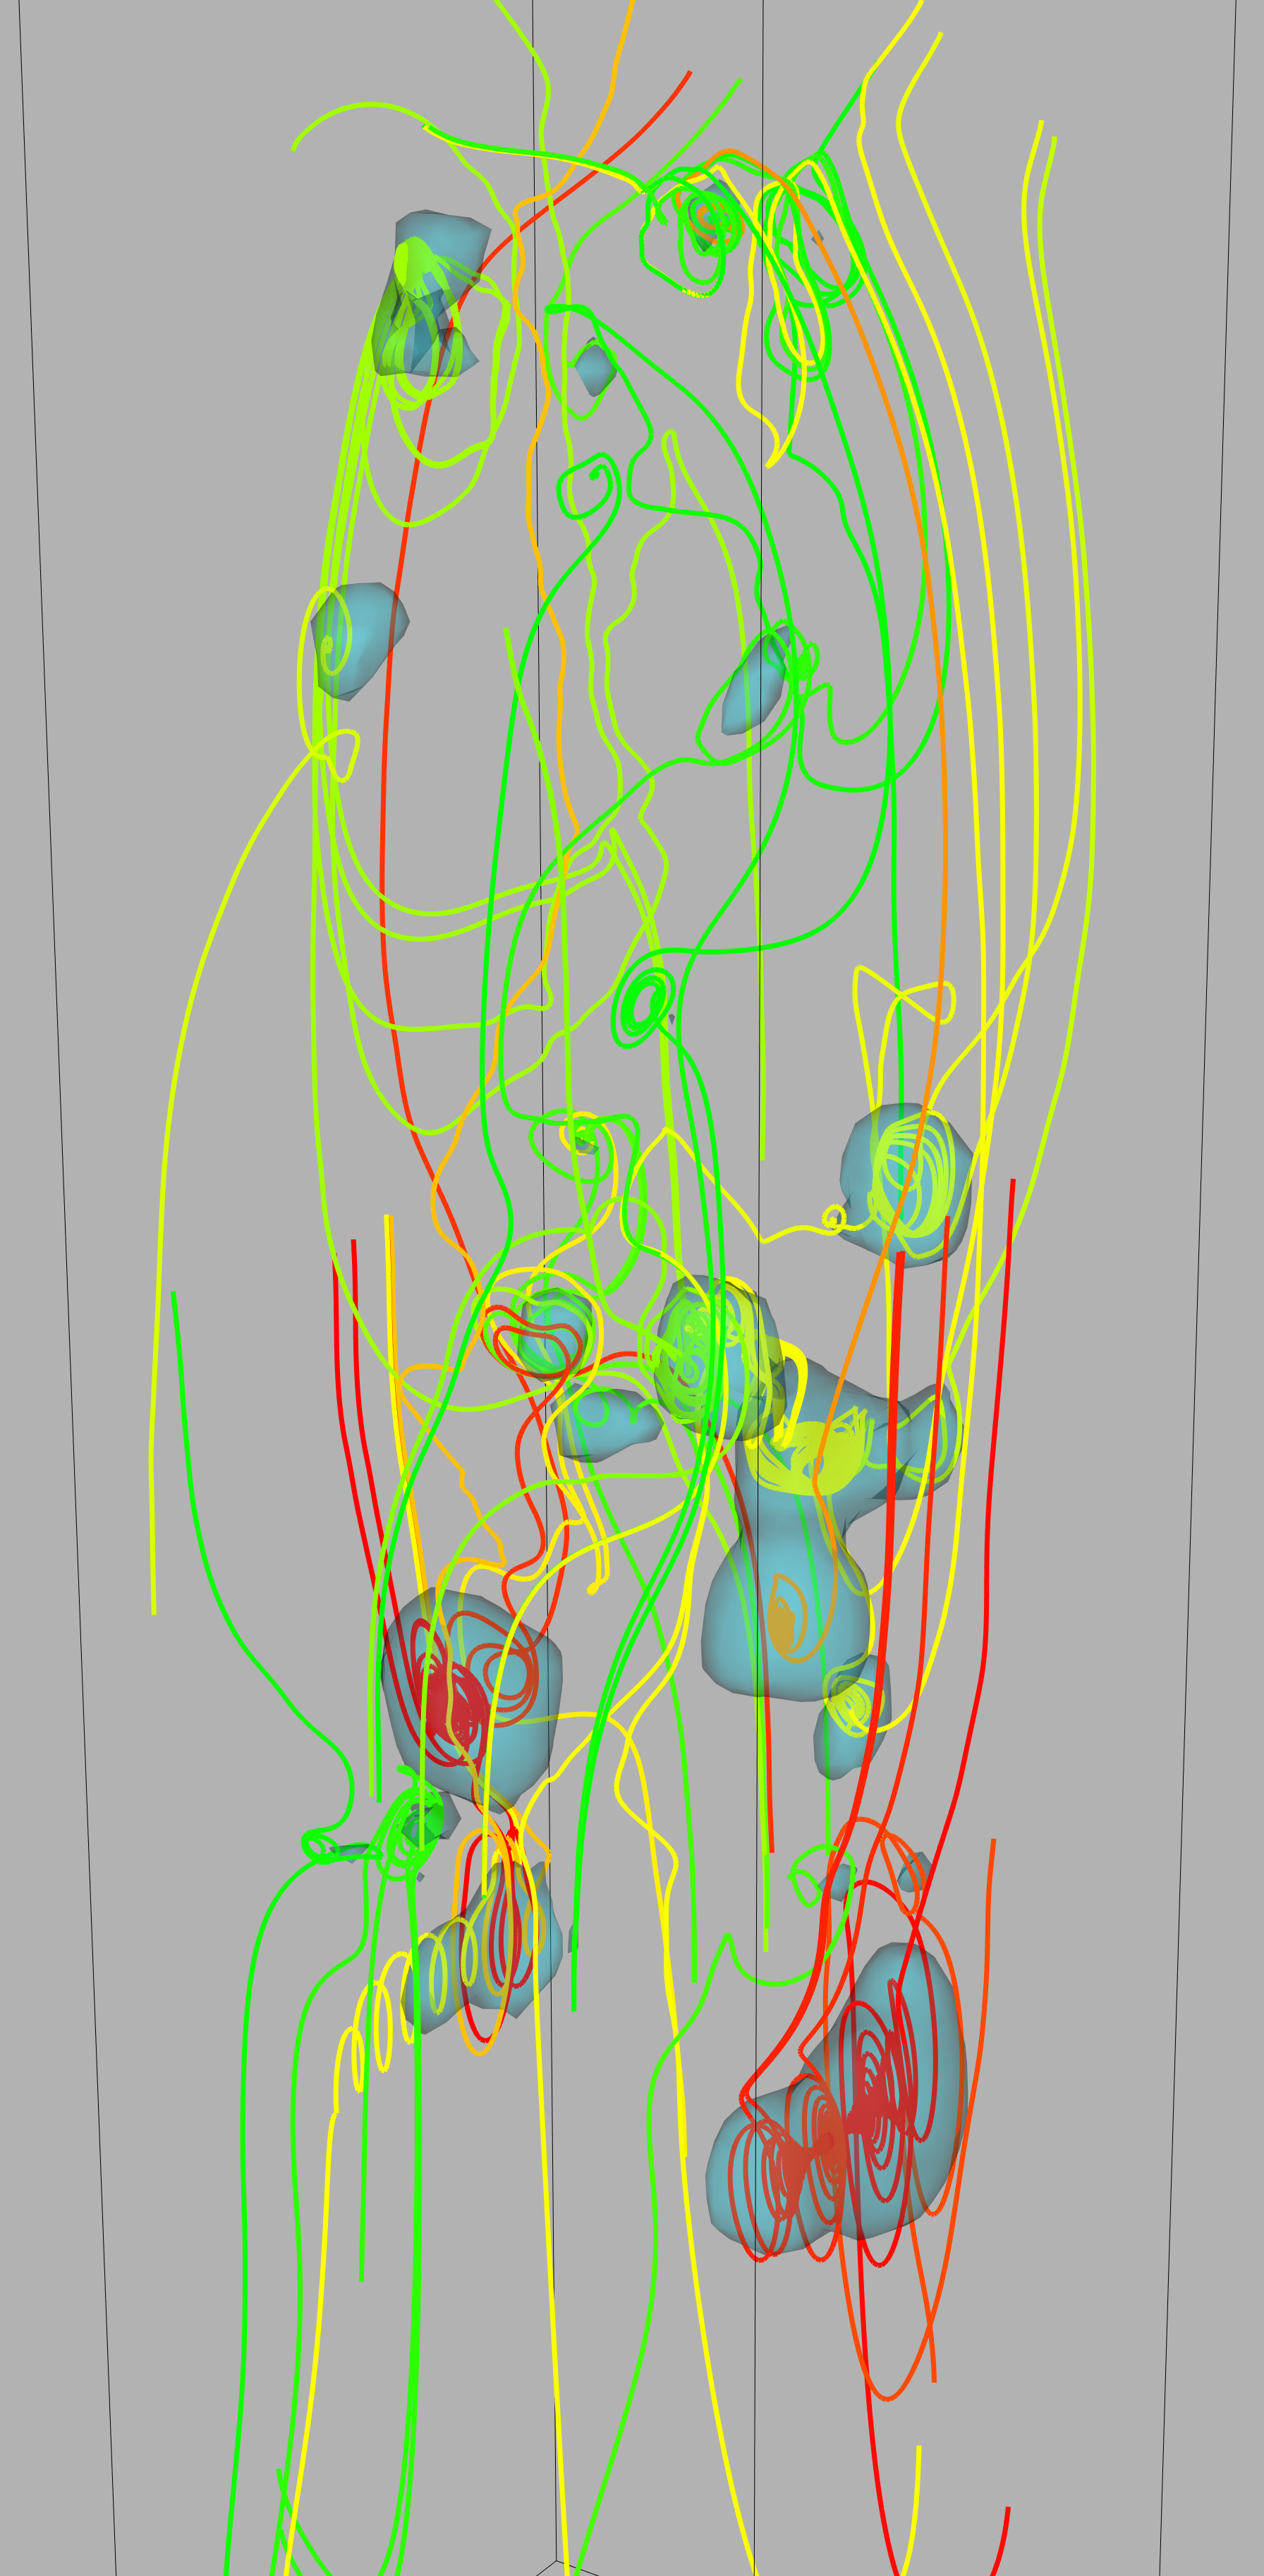
\includegraphics[height = 2\linewidth]{Images/plume_iso_crop.png}\\(b) The Solar Plume streamlines filtered by complexity mesasurements. \vspace{0.2em}
                \end{minipage}
        \caption{Example of how filtering increases the visibility of flow field features in the Solar Plume data set. In (a), the severe occlusion prevents any the viewer from seeing any structure in the flow field. (b) contains the same data set of streamlines as in (a), but with the filtering by complexity values applied. The number of streamlines has been significantly reduced and regions of high complexity are now clear to the viewer. Additionally, vortices in the flow field are enclosed by isosurfaces in (b).}
        \label{fig:plume_lines}
\end{figure}

Additionally, other visualization techniques are able to be applied to the plume data set.
The color plane allows the viewer to see that the Solar Plume plume consists of a mostly smooth behavior towards its center and then becomes more turbulent near to edges.
Rather than manually attempting to identify which regions of the flow field exhibit specific types of behavior, this visualization allows the viewer to identify these regions quickly.
A plane can be rendered to show the complexity values of the scalar field and the gradient isosurfaces can be rendered to show the areas of high change of turbulence.
These additional feautres for the Solar Plume data set are displayed in Fig \ref{fig:plume_additional}

\begin{figure}[h]
        \centering
                \begin{minipage}{0.47\linewidth}
                        %%\centering \small
                        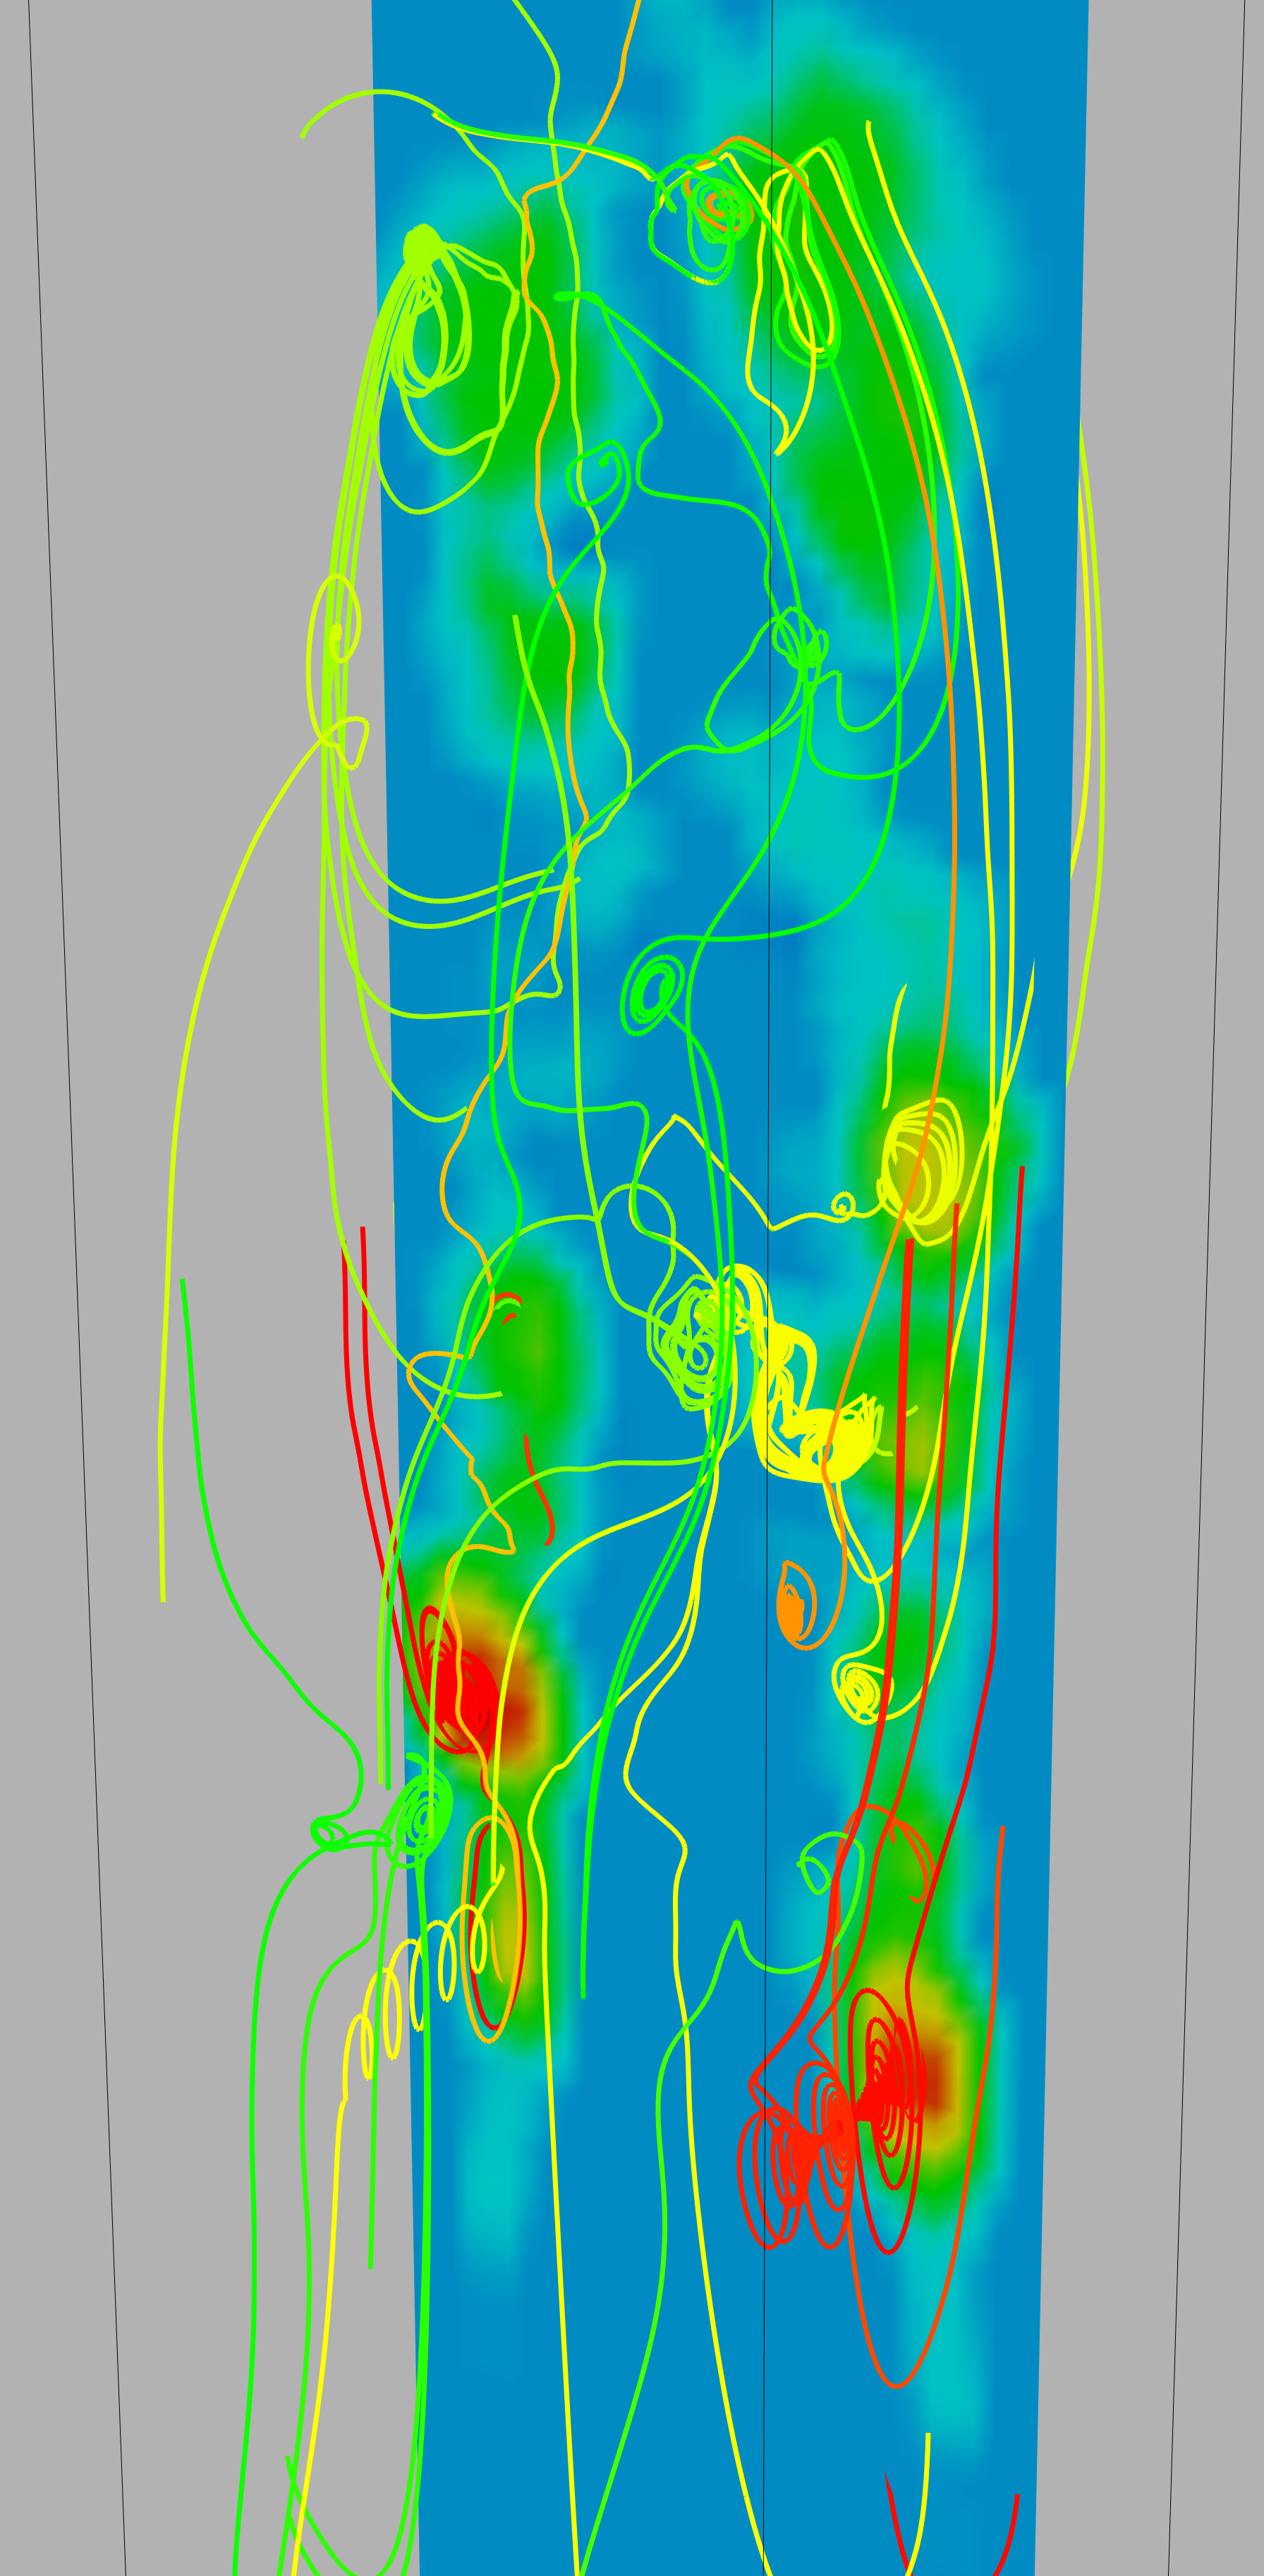
\includegraphics[height = 2\linewidth]{Images/plume_plane_crop.png}\\(a) High complexity areas highlighted by the colored plane. \vspace{0.2em}
                \end{minipage}
                \begin{minipage}{0.47\linewidth}
                        %%\centering \small
                        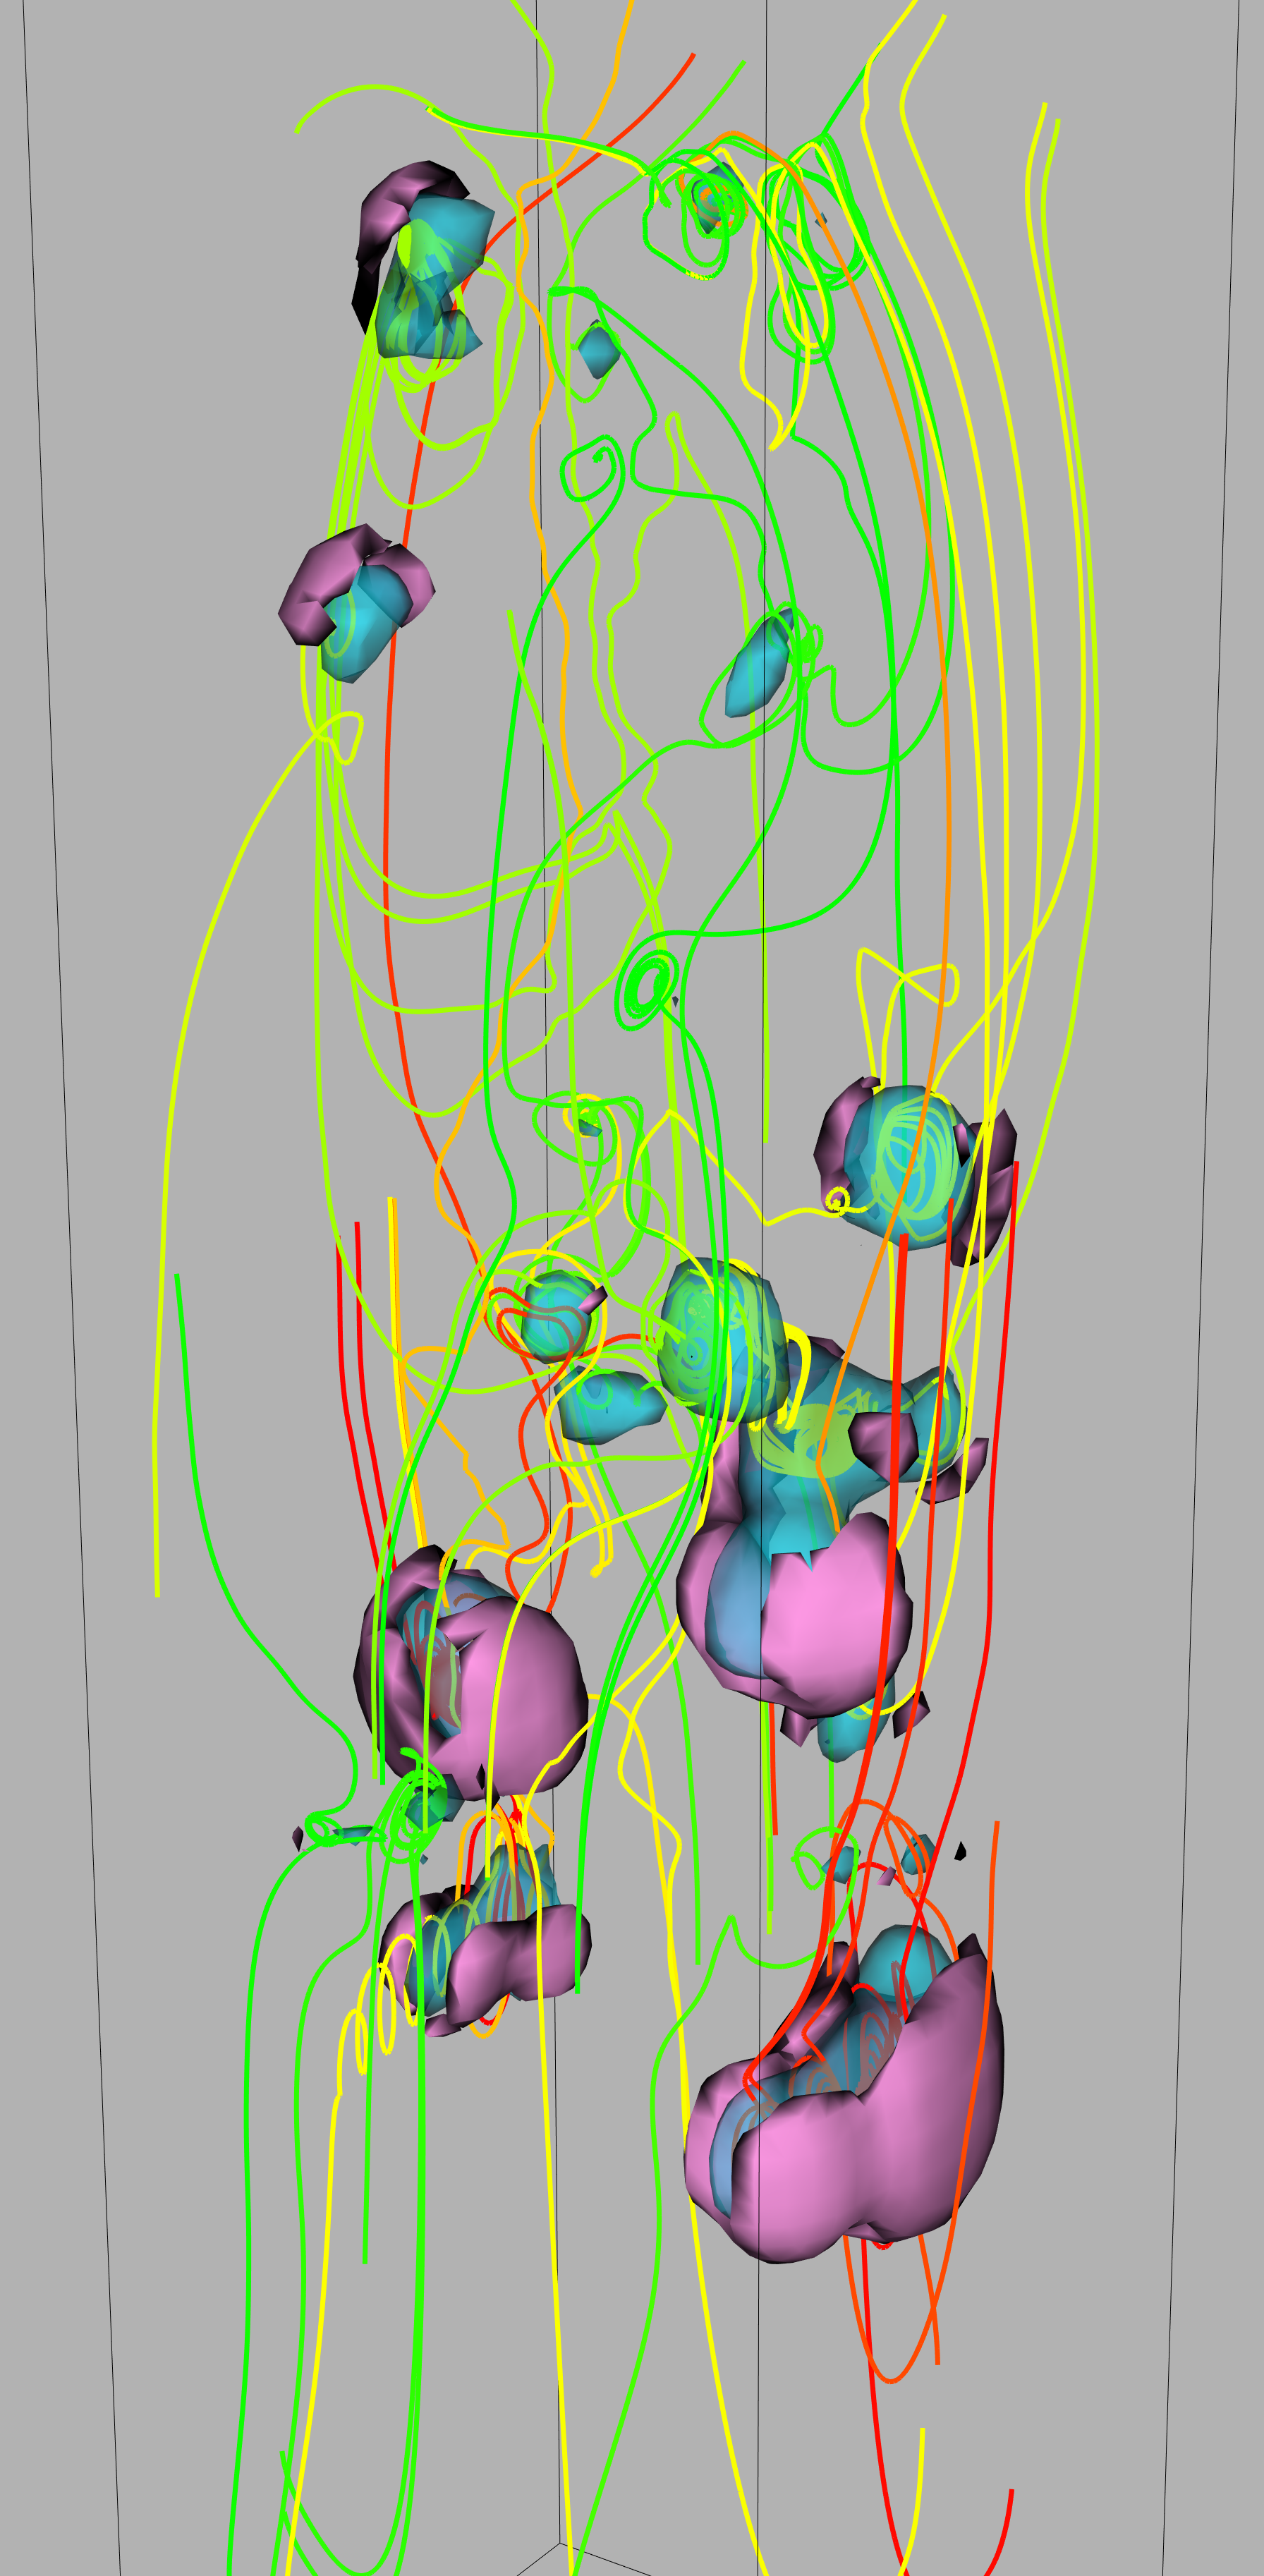
\includegraphics[height = 2\linewidth]{Images/plume_grad_crop.png}\\(b) Regions of high complexity change highlighted by an isosurface. \vspace{0.2em}
                \end{minipage}
        \caption{Example of additional visualization techniques in the Hurricane Isabel data set. In (a), the plane allows the viewer to see the different regions of high and low complexity. The gradient magnitude isosurfaces are displayed in (b). The isosurfaces form a boundary around the voritces in the plume data set.}
        \label{fig:plume_additional}
\end{figure}

A histogram with streamline complexity values are shown in Fig. \ref{fig:histogram}.
The histogram shows further examples from the Solar Plume data set of streamlines at different complexity values.
As the complexity value increases, the streamline becomes much less common and more difficult to find without a strategic method of filtering.


\begin{figure*}[t]
        \centering
                \begin{minipage}{0.99\linewidth}
                        \centering \small
                        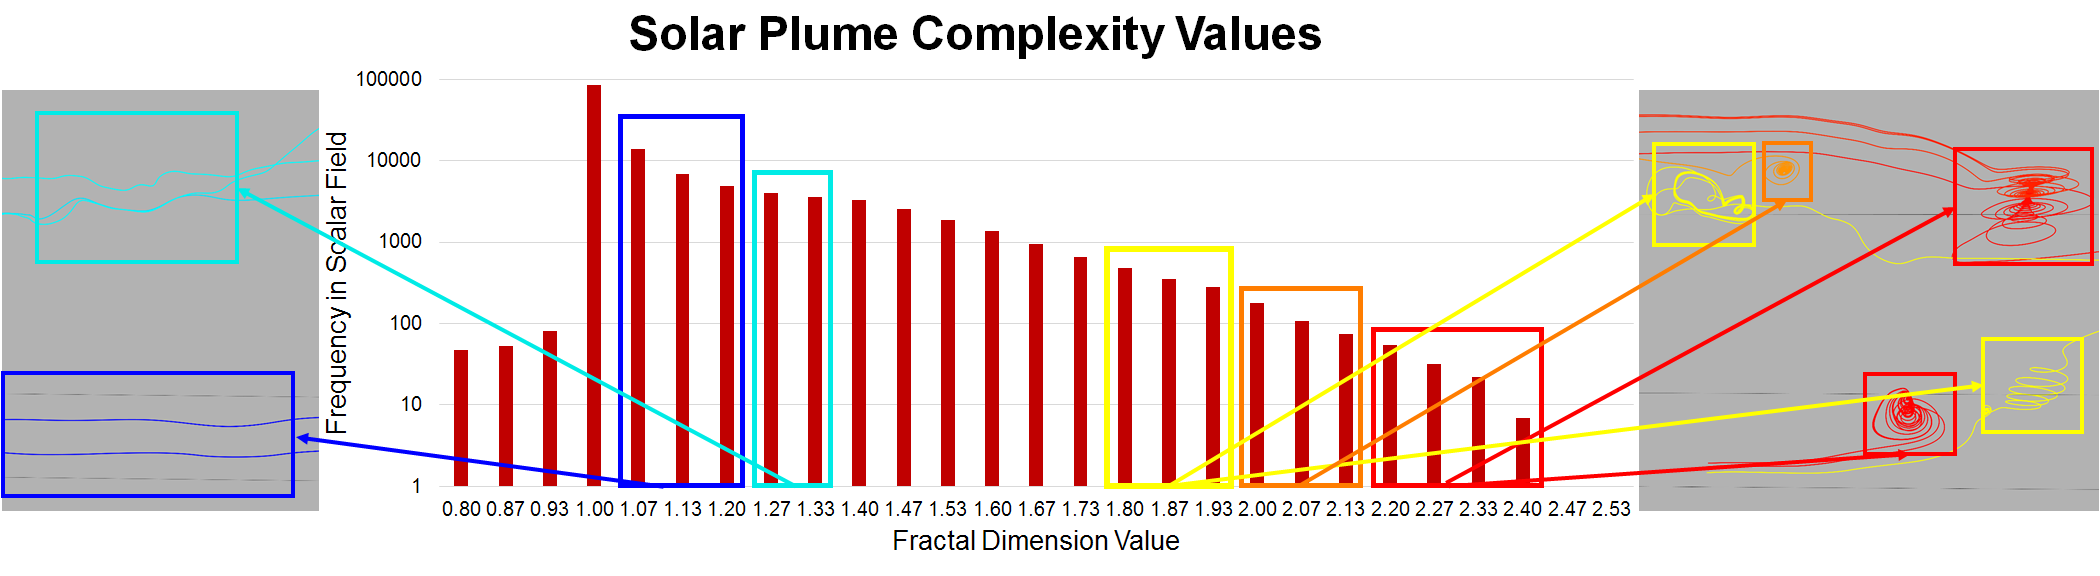
\includegraphics[height = .27\linewidth]{Images/histogram.png}
                \end{minipage}
        \caption{Histogram of different complexity values and examples of streamlines at those different complexity values.}
        \label{fig:histogram}
\end{figure*}

\subsection{Hurricane Isabel}

The Hurricane Isabel data set is a $500 \times 500 \times 100$ and used as a data set in a 2005 IEEE Visualization contest.
The data set consists of a mostly laminar flow along with several different isolated vortices within the flow.
Again, our algorithm is able to seperate these regions and highlight the significant sections to a view.

A regular sampling of streamlines from the Hurricane Isabel data set is displayed in Fig. \ref{fig:isa_lines}.a.
Without additional filtering, a viewer is not able to identify different or interesting portions of the flow field.
Our filtering algorithm was applied to the set of streamlines and the results of our filtering is displayed in Fig. \ref{fig:isa_lines}.b.
Again, the filtering is able to drastically reduce the clutter and make the significant parts of the flow field more visible to the viewer.
We are using the local maximum filtering and only showing streamlines with complexity values over 1.4.
The streamlines are again being colored by complexity and the isosurface is enclosing the portions of streamlines that have a complexity measurement of over 1.4.

\begin{figure}[h]
        \centering
                \begin{minipage}{1\linewidth}
                        %%\centering \small
                        \includegraphics[height = .62\linewidth]{Images/isa_all_crop.png}\\(a) The Hurricane Isabel streamlines seeded regularly through the flow field. \vspace{0.2em}
                \end{minipage}
                \begin{minipage}{1\linewidth}
                        %%\centering \small
                        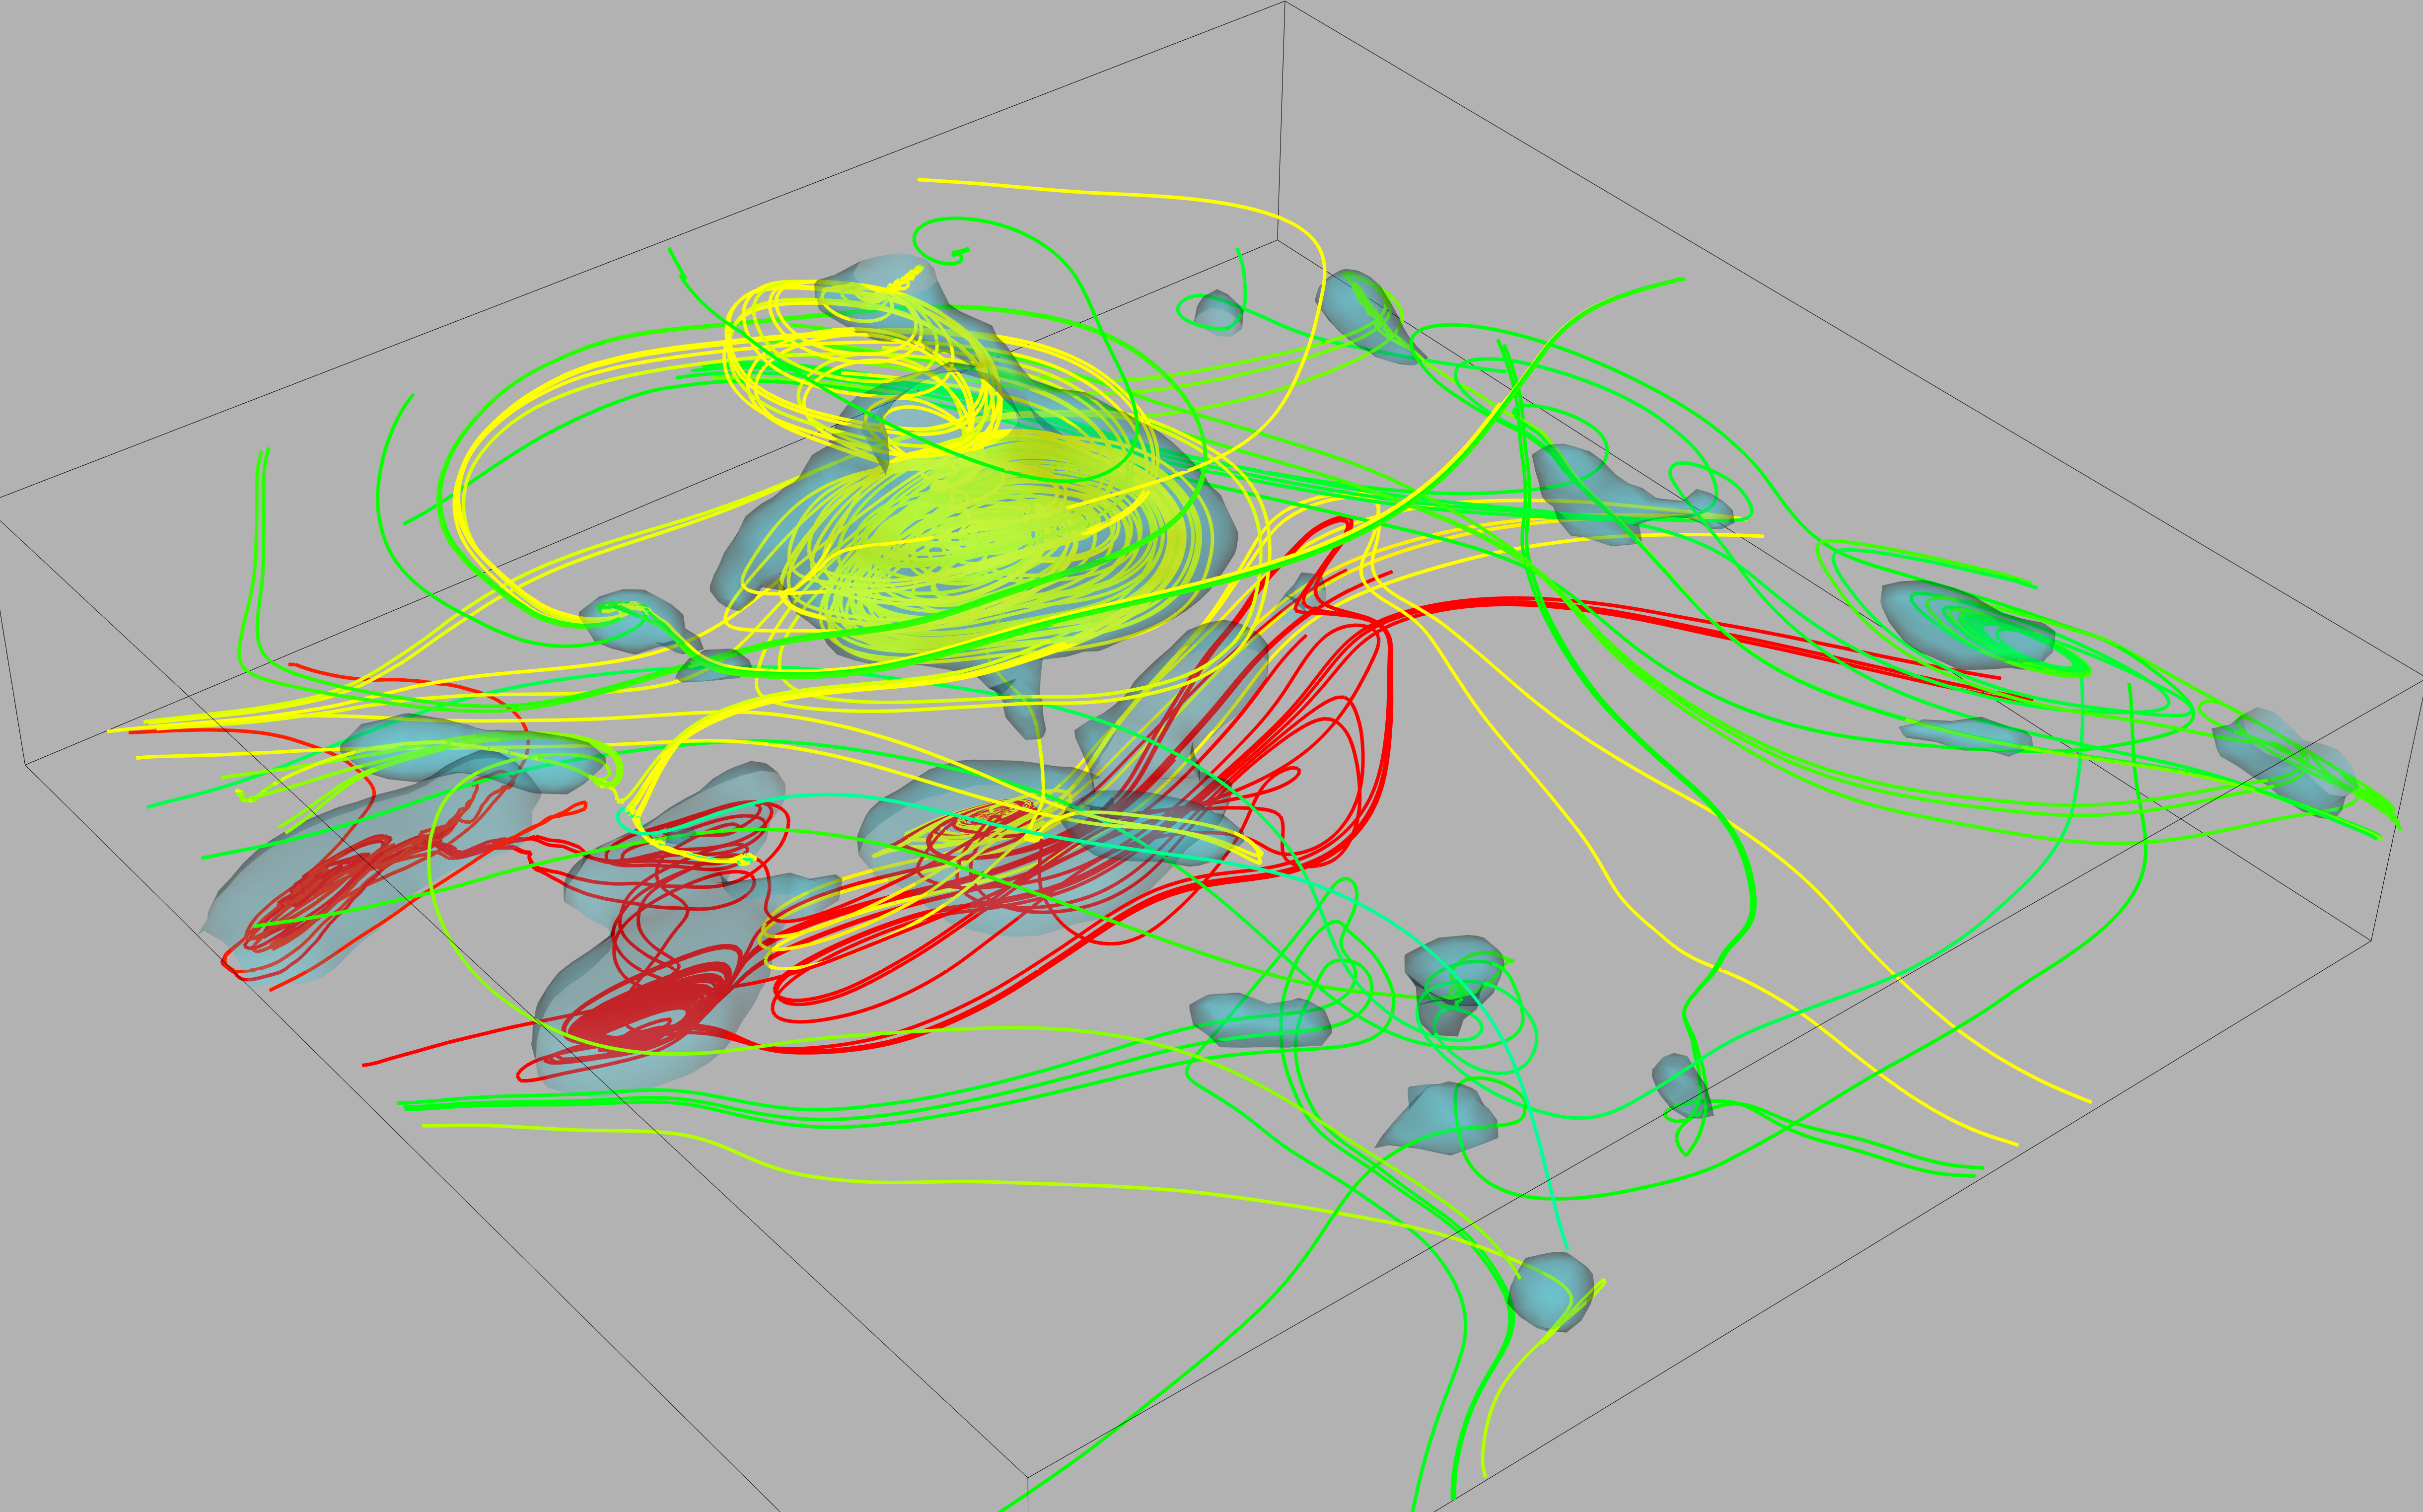
\includegraphics[height = .62\linewidth]{Images/isa_iso_crop.png}\\(b) The Hurricane Isabel streamlines filtered by complexity mesasurements. \vspace{0.2em}
                \end{minipage}
        \caption{Example of how filtering increases the visibility of flow field features in the Hurricane Isabel data set. In (a), the visualization is taken over by the simple, laminar streamlines. (b) contains the same data set of streamlines as in (a), but with the filtering by complexity values applied. The streamlines have now been significantly filtered so that the vortices in the data set are highlighted. These vortices are highlighted by isosurfaces.}
        \label{fig:isa_lines}
\end{figure}

Additional visualization methods also provide useful information in the flow visualization.
A colored plane visualization and the gradient isosurfaces are shown for the Hurricane Isabel data set in \ref{fig:isa_lines}.
The colored plane highlights three main regions of complexity near the red streamlines.
The gradient isosurface has an isosurface near .055 and mainly highlights the red vortices.

\begin{figure}[h]
        \centering
                \begin{minipage}{1\linewidth}
                        %%\centering \small
                        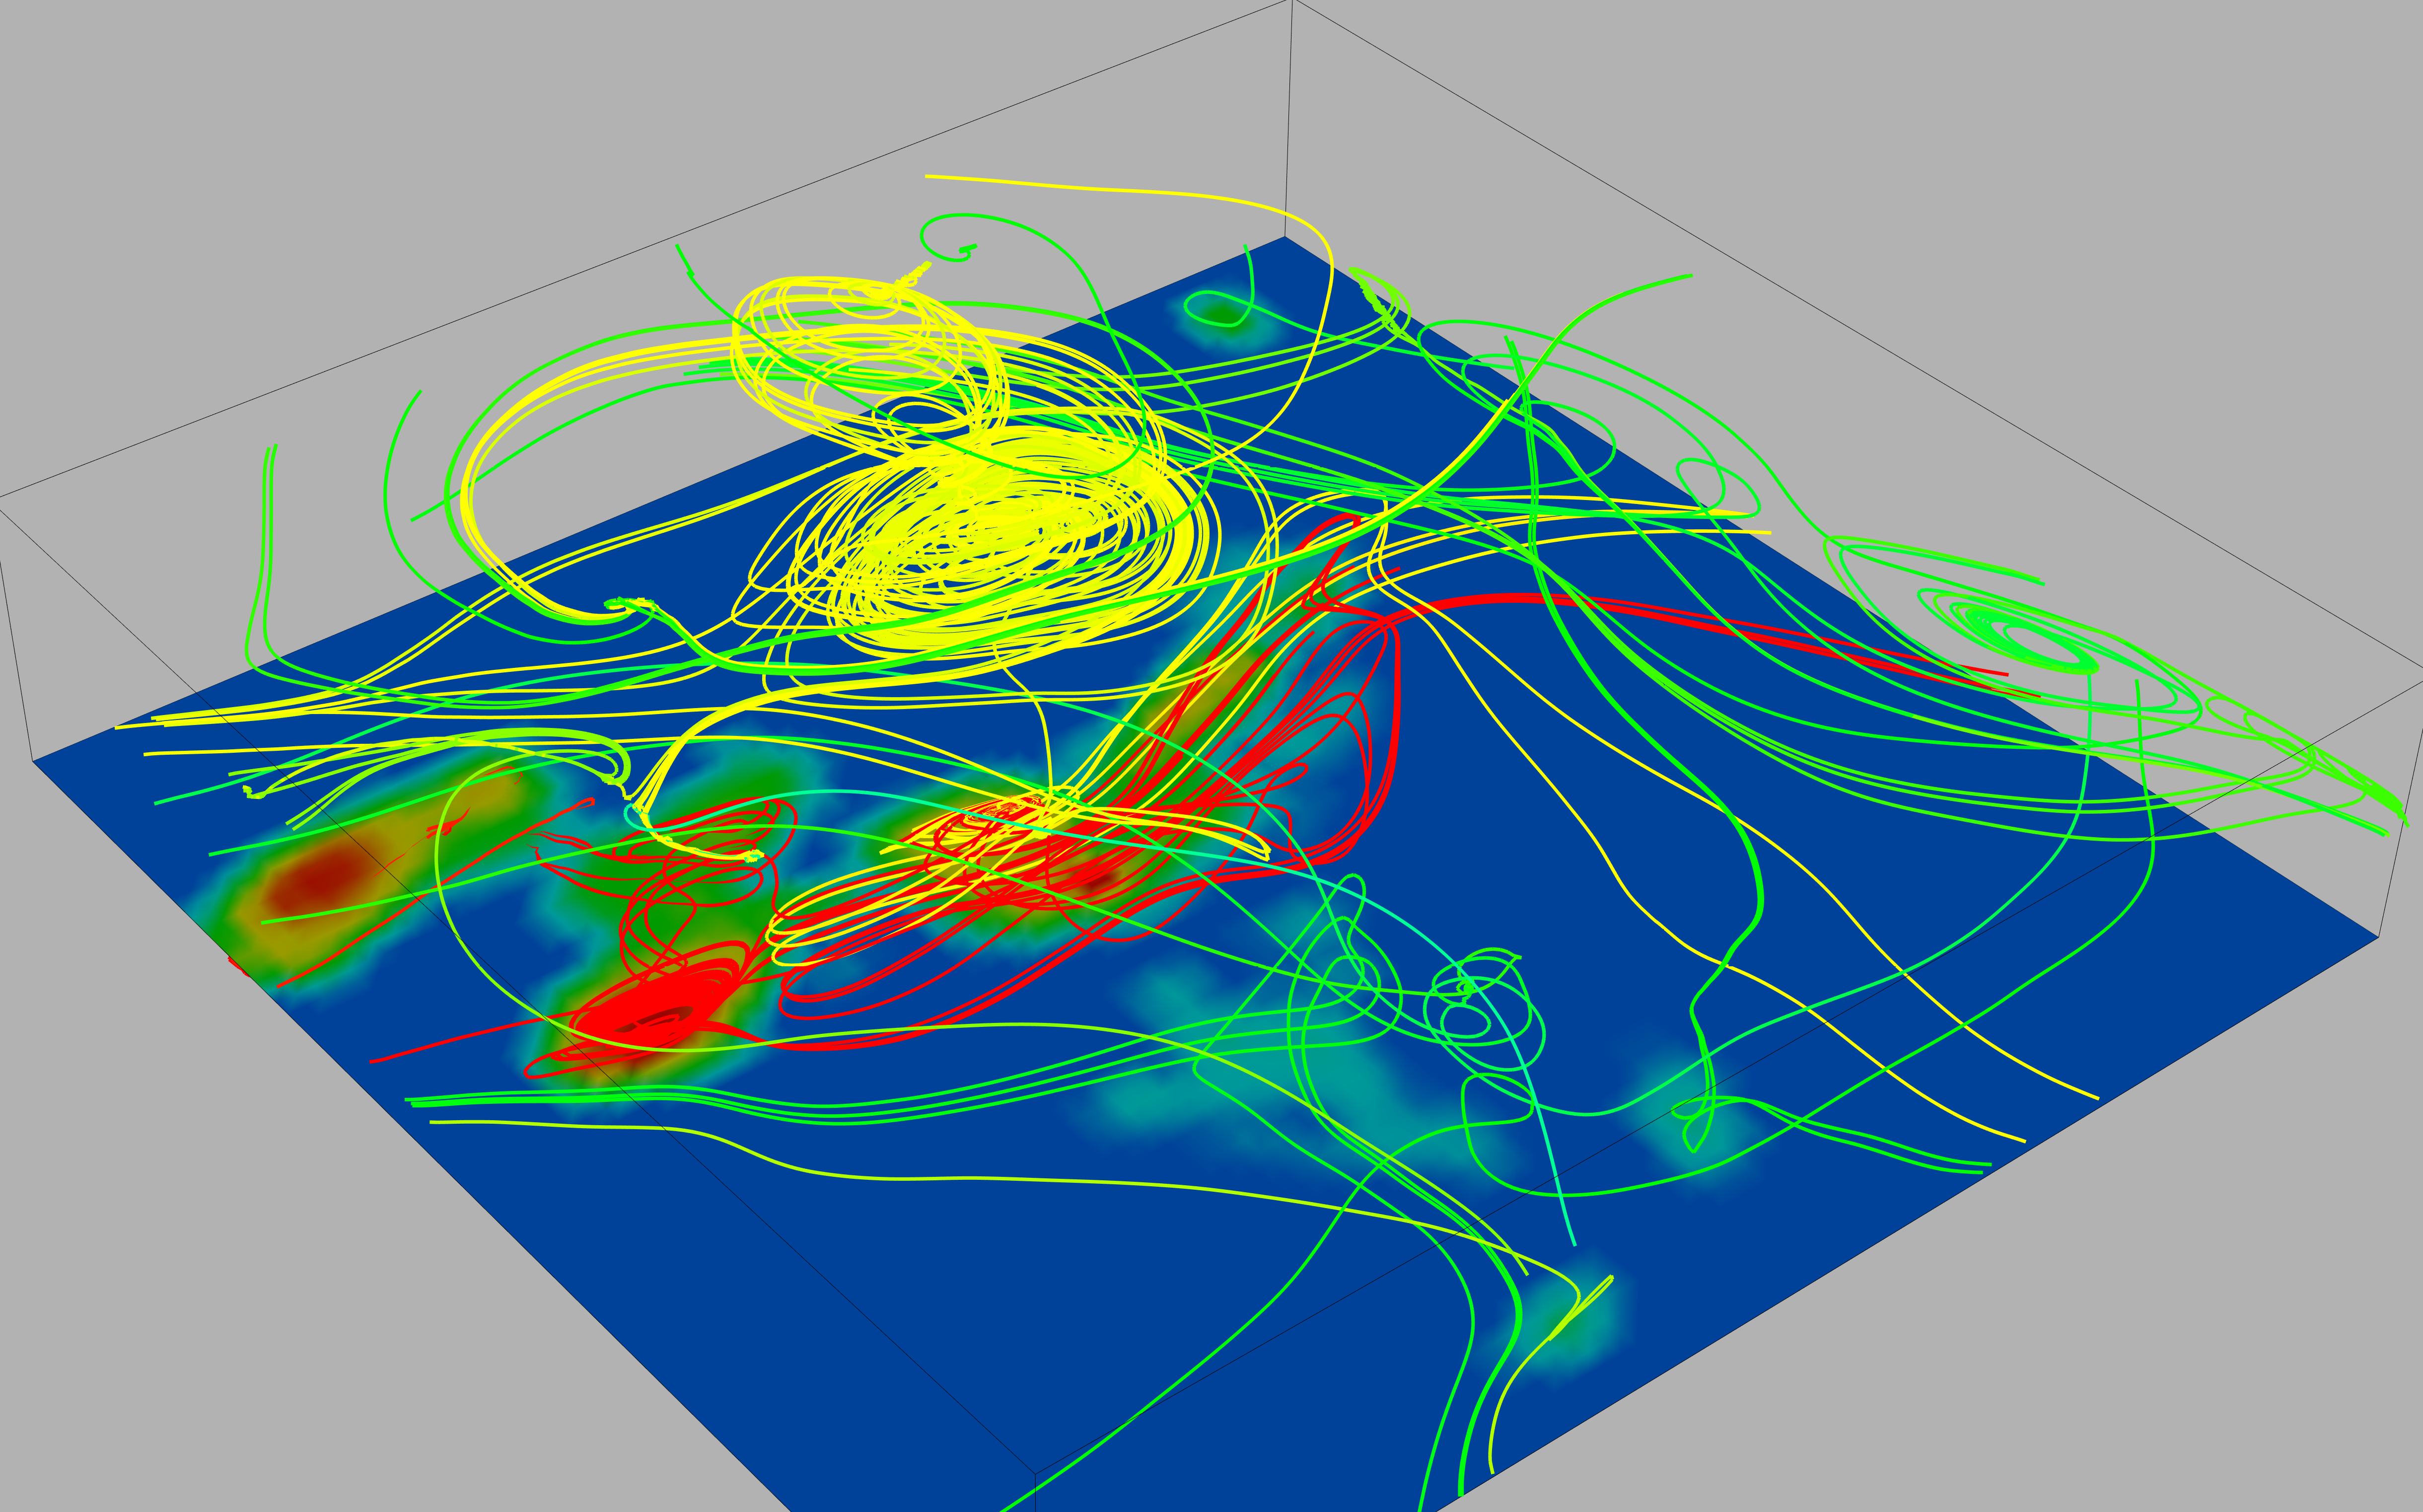
\includegraphics[height = .62\linewidth]{Images/isa_plane_crop.png}\\(a) High complexity areas highlighted by the colored plane. \vspace{0.2em}
                \end{minipage}
                \begin{minipage}{1\linewidth}
                        %%\centering \small
                        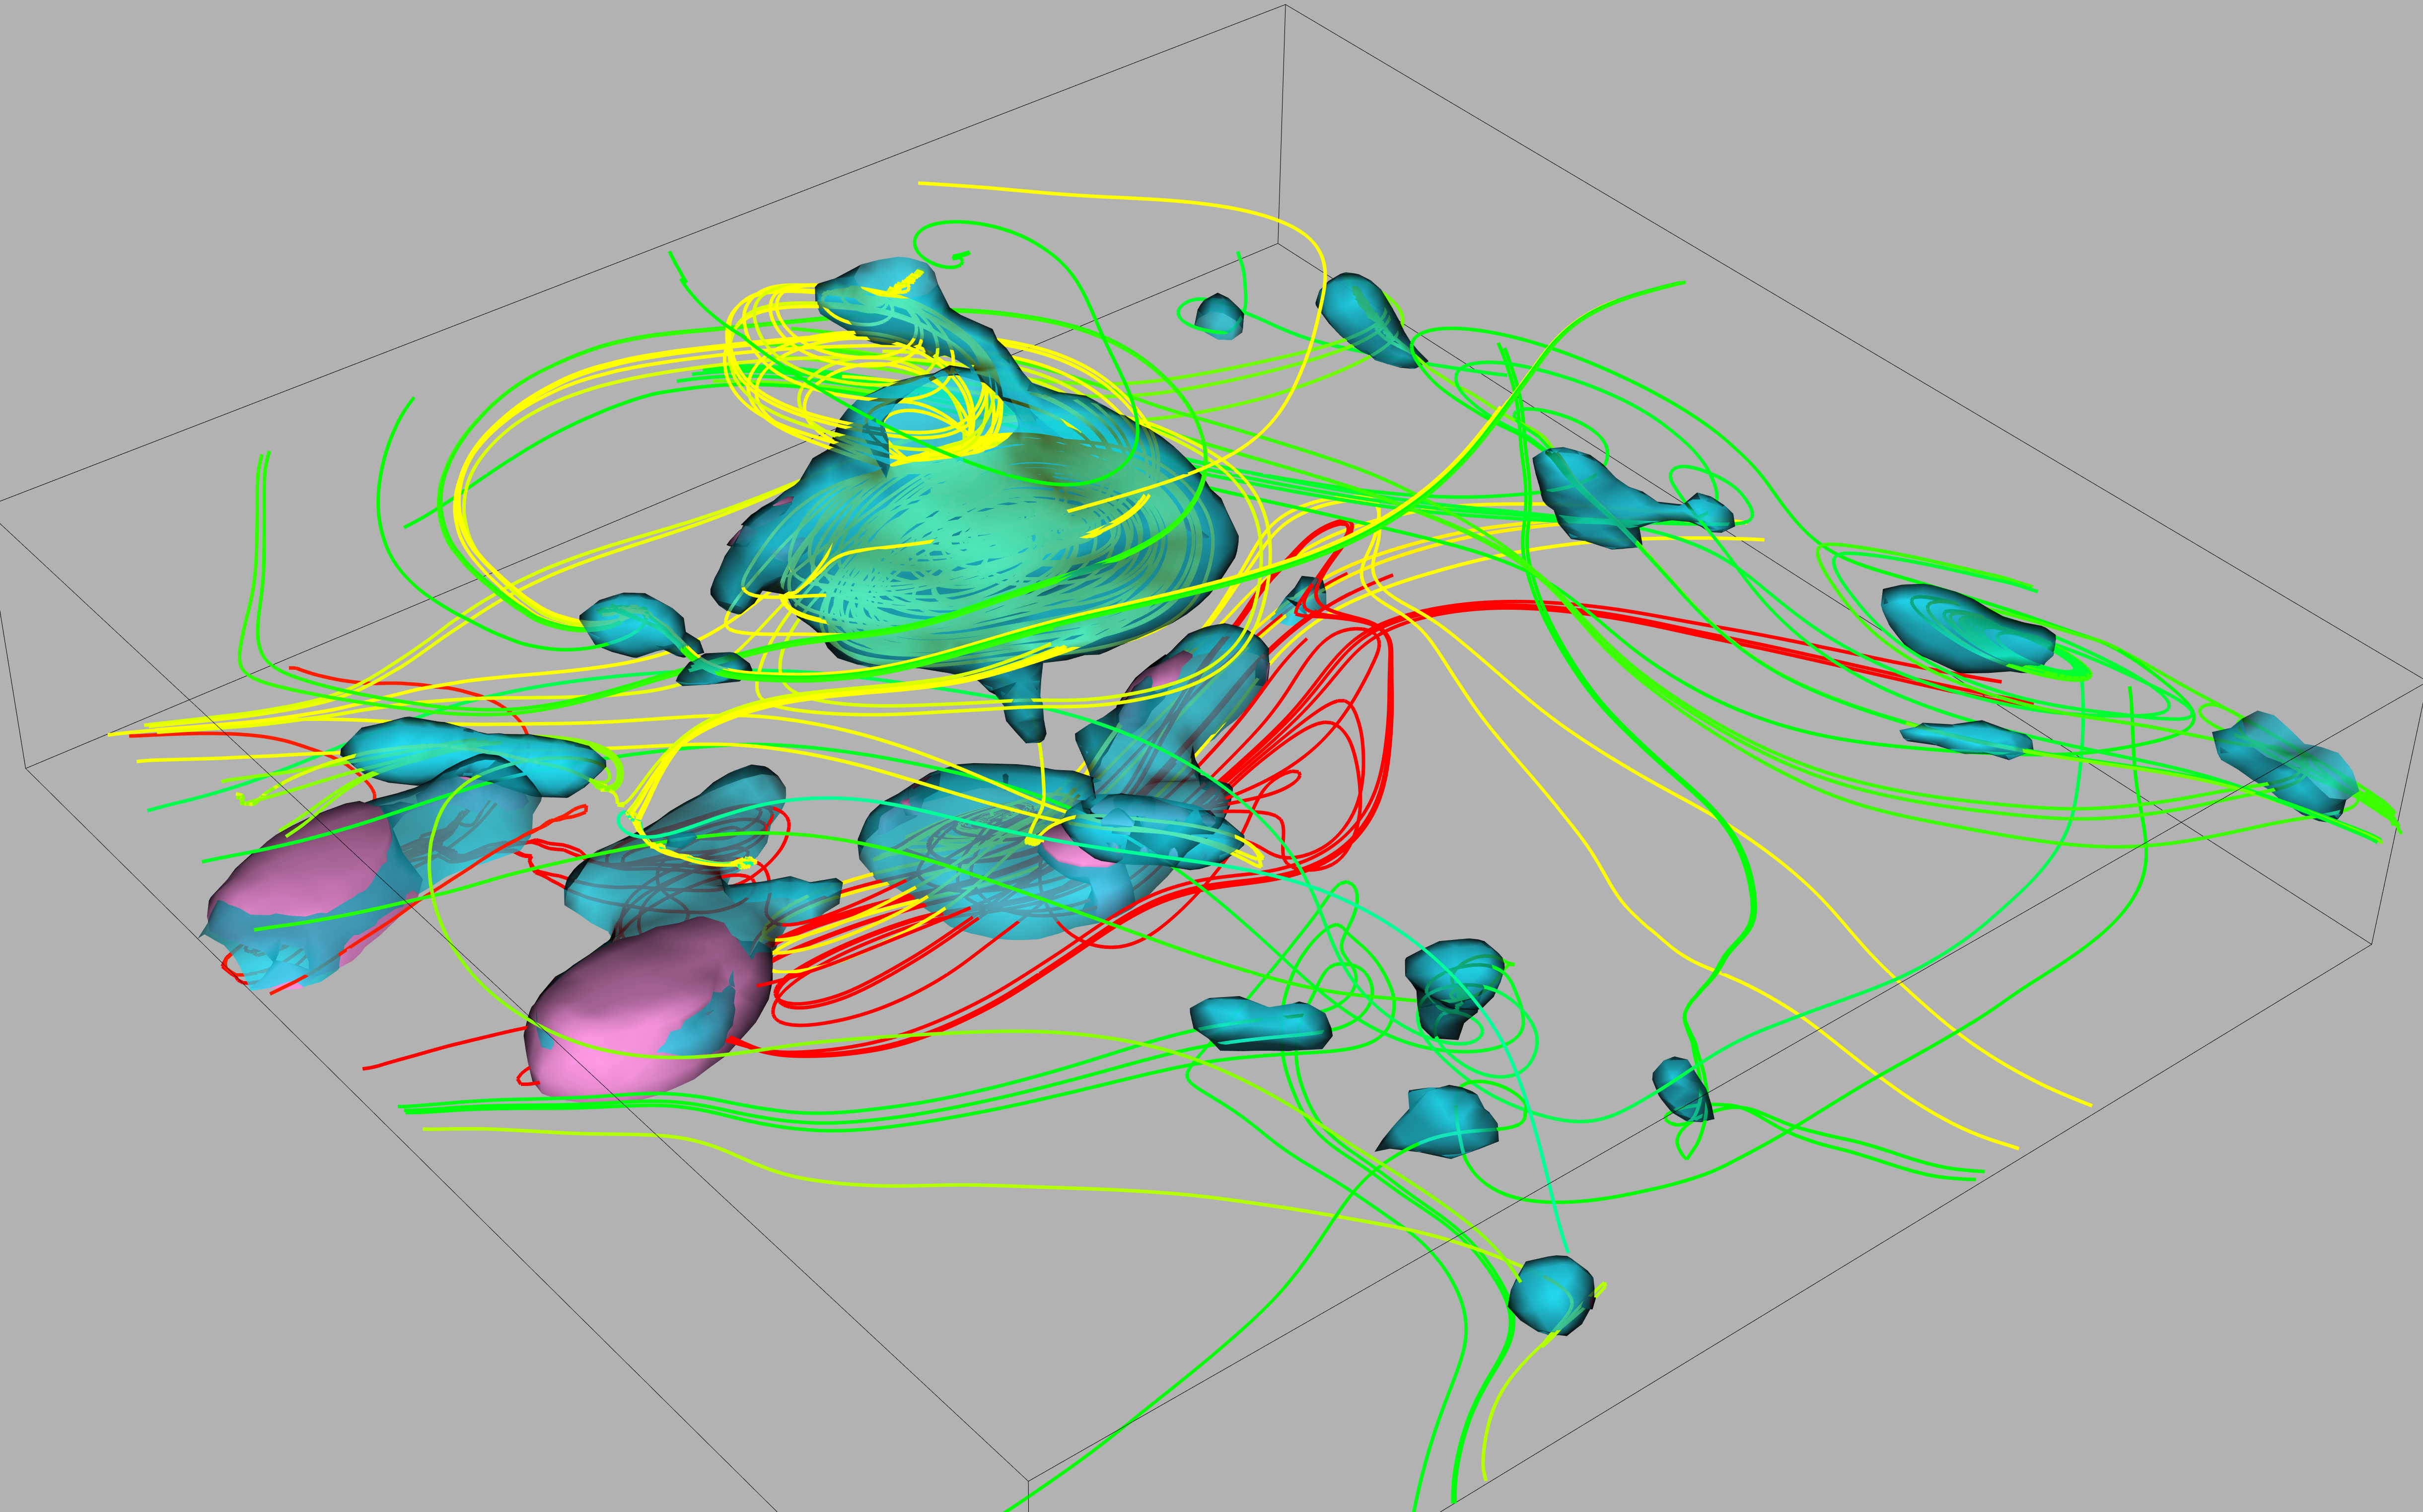
\includegraphics[height = .62\linewidth]{Images/isa_grad_crop.png}\\(b) Regions of high complexity change highlighted by an isosurface. \vspace{0.2em}
                \end{minipage}
        \caption{Example of additional visualization techniques for the Hurricane Isabel data set. The plane in (a) is situated near the bottom of the rendered flow field and highlights areas of varying flow complexity. The gradient magnitude isosurfaces are displayed in (b). The gradient isosurfaces specifically highlight the two red vortices which have the quickest complexity change.}
        \label{fig:isa_lines}
\end{figure}

\section{Evaluation} \label{sec:evaluations}

The complexity measurements for the streamlines are controlled by many parameters supplied by the user. 
In this section, we compare the complexity grids generated at different given values.
The user should be able to slightly change values without having the results be changed drastically.
It would be an invonnvenience to the user to require an exact set of values to produce reasonable results.
For this evaluation, we take a single reasonable input, and then slightly modify each value of the input and examine how that changes the scalar grid.

The original input has a spacing in the vector field of 4, uses a window size of 24, and has cutoff values for the box counting dimensions of 8.
All of the comparisons will be done off of the scalar grid that was generated from this data set.
The comparison is performed by taking the points in the original scalar grid and then finding the difference in the corresponding point in the other scalar grid.
In the tables (Fig. \ref{fig:v_gap}, \ref{fig:cutoff}, and \ref{fig:window_width}) below, we display how the values were changed as well as the mean difference between the scalar grids and the standard deviation of the differences.

\begin{figure}[h]
\begin{tabular}{|l|l|l|}
   \hline
    Vector space & Mean difference  & Standard deviation\\
    \hline
2&0.0720&0.0668\\
4&0.0000&0.0000\\
5&0.0644&0.0612\\
6&0.0761&0.0653\\
7&0.0856&0.0708\\
8&0.0875&0.0735\\
16&0.1340&0.0957\\
     \hline
\end{tabular}
\caption{Comparison of different spaces between the regularly seeded vectors.}
\label{fig:v_gap}
\end{figure}

\begin{figure}[h]
\begin{tabular}{|l|l|l|}
   \hline
    Cutoff value & Mean difference  & Standard deviation\\
    \hline
2&0.0943&0.0922\\
3&0.0953&0.0933\\
4&0.0920&0.0890\\
6&0.0835&0.0814\\
8&0.0000&0.0000\\
10&0.1181&0.1206\\
13&0.1553&0.1298\\
17&0.1790&0.1258\\
     \hline
\end{tabular}
\caption{Comparison of different cutoff values in the box counting dimension.}
\label{fig:cutoff}
\end{figure}

\begin{figure}[h]
\begin{tabular}{|l|l|l|}
   \hline
    Window width & Mean difference  & Standard deviation\\
    \hline
16&0.1812&0.1281\\
24&0.0000&0.0000\\
28&0.1002&0.0833\\
32&0.1001&0.0822\\
36&0.1215&0.0918\\
40&0.1221&0.0926\\
     \hline
\end{tabular}
\caption{Comparison of different window widths used in the box counting dimension.}
\label{fig:window_width}
\end{figure}

The tables show that the user has a reasonable window in which parameters can be altered without drastically altering the scalar field values.
(Not sure what to say about this or if these values are even low enough).

\section{Summary and Future Work}

In this paper we propsed a method of filtering streamlines and identifyingn complex regions of the flow field.
We descibed a method of box counting dimension for streamlines to identify the streamlines that have a space filling pattern and are complex.
Then using this box counting dimension, we are able to make a streamline complexity grid that has scalar values to represent the complexities of different regions.
The streamline complexity grid along with the streamline box counting dimensions allow for many visualization techniques such as filtering by local maximums and isosurfaces to allow the viewer to identify interesting parts of a flow field.
We then appleid these filtering methods and visualization techniques to various data set and showed how they created a quality visualization.

One additional application of the streamline complexity grid could possibly be determining the opacities to assign regions in 3D Line Integral Convolution.
In 3D Line Integral Convolution, if regions are not strategically given varying opacities, the volume cannot be seen due to occlusion.
One can reasonably want to make the less transparent regions have a high opacity and the more complexity regions have a lower opacity.
The streamline complexity grid could potentially aid in this area.

We also plan to investiage stream surfaces with the box counting ratio and streamline complexity grid.
We plan to apply our definition of the box counting ratio to stream surfaces generated from the flow field as well to identify interesting or complexity stream surfaces.
Also, we intend to investigate if the streamline complexity grid can act as a guide in placing stream surfaces.
Generating stream surfaces is fundamentally more difficult that generating streamlines because a curve must also be defined for the stream surface, which makes brute force searching methods unreasonable.
We will attempt to use the streamline complexity grid to identify regions to search for the placement of stream surfaces.

%\bibliographystyle{eg-alpha}
\bibliography{fractalFlow}
\bibliographystyle{eg-alpha-doi}


\end{document}
